% Online Resource 1 for Computational Statistics; 25 October 2026
\documentclass[11pt,a4paper]{article}
\usepackage[margin=23mm]{geometry}
\usepackage{graphicx,amsmath,amssymb,bm,booktabs,placeins}
\usepackage{caption}
\captionsetup[figure]{name=Fig.,labelfont=bf,labelsep=space}
\usepackage[authoryear,round]{natbib}
\usepackage{xr}
\externaldocument[][nocite]{article}
\usepackage[hidelinks]{hyperref}
\hypersetup{pdftitle={Online Resource 1: Gated Cluster-Pooled Sign Constraints for Multi-Output Sparse Regression},
pdfauthor={Artur Sepp and Mika A. Kastenholz}}
\providecommand{\bibcommenthead}{}
\renewcommand{\thesection}{S\arabic{section}}
\renewcommand{\theequation}{S\arabic{equation}}
\renewcommand{\thetable}{S\arabic{table}}
\renewcommand{\thefigure}{S\arabic{figure}}
\setcounter{tocdepth}{2}
\makeatletter
\renewcommand{\l@section}{\@dottedtocline{1}{0em}{2.8em}}
\renewcommand{\l@subsection}{\@dottedtocline{2}{2.8em}{3.8em}}
\makeatother
\title{Online Resource 1\\[0.5em]\large Gated Cluster-Pooled Sign Constraints for Multi-Output Sparse Regression}
\author{Artur Sepp and Mika A. Kastenholz\\\small LGT Bank, Quantitative Analytics\\\small Bleicherweg 30, 8002 Zurich, Switzerland\\\small Correspondence: \texttt{artur.sepp@lgt.com}}
\date{Computational Statistics submission materials, 25 October 2026}
\begin{document}
\maketitle
This supplement supplies mathematical details, complete study protocols,
extended results and computational checks for the main article. The previously
verified results are retained, with a further variance-convention sensitivity
comparison in Section~\ref{app:variance-sensitivity} and a Monte Carlo check of
the pooling precision formula in Section~\ref{app:precision-check}. The record of
historical conventions and corrections is kept with Online Resource~2.
Figures were produced with Python and Matplotlib.
\tableofcontents
\clearpage
\section{Conditions and proof for the on-support gate result} \label{app:theory}

The result below concerns the sign matrix produced by the date-score gate, not
the support or distribution of the fitted coefficient matrix. It allows
contemporaneous response dependence and random response clusters, with a
structural assumption on which clusters can be selected asymptotically. The
number of predictors and responses is fixed.

Let $(\bm x_t,\bm y_t)$ denote population-centered observations and let
$\bm\beta_{\mathrm{true}}$ be the coefficient matrix in
$\bm y_t=\bm\beta_{\mathrm{true}}\bm x_t+\bm\varepsilon_t$.
For any nonempty response subset $\mathcal C$, write
$m=|\mathcal C|$, $\bar y_{t,\mathcal C}=m^{-1}\sum_{k\in\mathcal C}y_{tk}$,
and define
\begin{equation}\label{eq:population-pooled-slope}
 q_j=E[x_{tj}^2],\qquad
 b_{j,\mathcal C}=\frac{E[x_{tj}\bar y_{t,\mathcal C}]}{q_j},\qquad
 \bar r_{t,j,\mathcal C}=\bar y_{t,\mathcal C}-b_{j,\mathcal C}x_{tj}.
\end{equation}
Here $b_{j,\mathcal C}$ is a population marginal slope, not an individual
partial coefficient. Define the population score scale
\begin{equation}\label{eq:gate-influence-variance}
 \omega_{j,\mathcal C}^2
 =q_j^{-2}E[x_{tj}^2\bar r_{t,j,\mathcal C}^{\,2}].
\end{equation}
With fixed analysis scales this is the marginal slope's influence variance.
When column scales are estimated from the same observations, additional
scale-estimation terms can enter the slope's centered limiting distribution.
The result below uses only the displayed positive score scale and makes no
calibrated-inference claim for that sample-normalized slope.
Let $\mathfrak C$ be a deterministic finite family of nonempty response
subsets. A pair $(j,\mathcal C)$ is called relevant if
$\beta_{\mathrm{true},kj}\ne0$ for at least one $k\in\mathcal C$.

\paragraph{Conditions.}
\begin{description}
 \item[(A1) Sampling and exogeneity.] The dates
 $(\bm x_t,\bm\varepsilon_t)$ are independent and identically distributed,
 $E[\bm x_t]=\bm0$, and
 $E[\bm\varepsilon_t\mid\bm x_t]=\bm0$. The matrix
 $\bm\beta_{\mathrm{true}}$ and dimensions $N,M$ do not vary with $T$.
 Response errors within a date may be dependent.
 \item[(A2) Moments, centering and analysis units.] Every component of
 $\bm x_t$ and $\bm\varepsilon_t$ has a finite fourth moment, and
 $\bm\Sigma_F=E[\bm x_t\bm x_t^\top]$ is positive definite.
 Only complete observations are used. If a column is standardized, its
 population variance is positive, and $\bm x_t,\bm y_t$ and
 $\bm\beta_{\mathrm{true}}$ denote the variables and coefficients in
 the corresponding population-standardized units. If a column is not
 standardized, it retains its specified fixed measurement units.
 Thus (A3), (A4) and (A6) refer to pooled marginal slopes in these limiting
 analysis units. Positive column rescaling preserves individual partial
 signs, but need not preserve a pooled marginal sign.
 The empirical columns are centered by their sample means. Write
 $\widehat s_{x,j},\widehat s_{y,k}$ for their further empirical scale
 factors in the limiting units: each is one for an unstandardized column
 and its sample standard deviation for a standardized column. Hence
 $\widehat s_{x,j}=1+O_p(T^{-1/2})$ and
 $\widehat s_{y,k}=1+O_p(T^{-1/2})$, as follows from the fourth moments
 and positive population variances.
 \item[(A3) Admissible clusters and coherence.] Let
 $\widehat{\mathcal P}_T$ be the supplied or estimated partition. The event
 $\mathcal E_T=\{\widehat{\mathcal P}_T\subseteq\mathfrak C\}$ has probability
 tending to one. Within every $\mathcal C\in\mathfrak C$ and for every
 predictor $j$, all nonzero $\beta_{\mathrm{true},kj}$ have the same sign.
 For a fixed supplied partition, $\mathcal E_T$ can hold identically.
 \item[(A4) Nondegenerate marginal signals.] For constants
 $\delta>0$ and $0<c<C<\infty$, every relevant pair with
 $\mathcal C\in\mathfrak C$ satisfies
 $|b_{j,\mathcal C}|\geq\delta$ and
 $c\leq\omega_{j,\mathcal C}^2\leq C$.
 This is a population signal condition; it does not assume that an estimated
 gate statistic has already passed its threshold.
 \item[(A5) Gate and threshold.] Use the complete-data, equal-weight statistic
 in Equation~\eqref{eq:date-score}. The deterministic threshold
 satisfies $\tau_T\geq0$ and $\tau_T=o(\sqrt T)$; any fixed finite threshold is
 included. No penalty-rate assumption is imposed.
 \item[(A6) Marginal sign agreement.] For every relevant
 $(j,\mathcal C)$ with $\mathcal C\in\mathfrak C$ and every nonzero
 $\beta_{\mathrm{true},kj}$ in that cluster,
 $\operatorname{sign}(b_{j,\mathcal C})
 =\operatorname{sign}(\beta_{\mathrm{true},kj})$.
\end{description}

Under exogeneity the marginal slope is
\begin{equation}\label{eq:marginal-leakage}
 b_{j,\mathcal C}
 =\frac{1}{m\,\Sigma_{F,jj}}
 \sum_{k\in\mathcal C}\sum_{\ell=1}^M
 \beta_{\mathrm{true},k\ell}\Sigma_{F,j\ell}.
\end{equation}
With uncorrelated predictors it is the average partial coefficient, so (A3)
implies (A6). With correlated predictors, the other terms can reverse its sign.
Condition (A3) is an assumption about the clustering procedure under the
data-generating law, not a consequence of positive response correlations.
Conditions (A3)--(A6) permit partially shared supports, but exclude cancellation
or sign reversals in the relevant population pooled slopes.

\paragraph{Lemma 1 (a sufficient condition for marginal-sign agreement).}
\label{lem:leakage-supp}
Assume (A1), (A2) and the coherence part of (A3) for a relevant pair
$(j,\mathcal C)$, with common sign $s\in\{-1,+1\}$ on its nonzero
$\beta_{\mathrm{true},kj}$. If
\begin{equation}\label{eq:leakage-condition-supp}
 \Sigma_{F,jj}\sum_{k\in\mathcal C}|\beta_{\mathrm{true},kj}|
 \;>\;
 \sum_{k\in\mathcal C}\sum_{\ell\ne j}
 |\beta_{\mathrm{true},k\ell}|\,|\Sigma_{F,j\ell}| ,
\end{equation}
then $\operatorname{sign}(b_{j,\mathcal C})=s$ and $|b_{j,\mathcal C}|$ is at
least the difference of the two sides of
Equation~\eqref{eq:leakage-condition-supp} divided by $m\,\Sigma_{F,jj}$.

\paragraph{Proof.}
Equation~\eqref{eq:marginal-leakage} separates into own-effect and leakage
terms,
\[
 m\,\Sigma_{F,jj}\,b_{j,\mathcal C}
 =\Sigma_{F,jj}\sum_{k\in\mathcal C}\beta_{\mathrm{true},kj}
 +\sum_{k\in\mathcal C}\sum_{\ell\ne j}\beta_{\mathrm{true},k\ell}\Sigma_{F,j\ell}.
\]
By coherence every nonzero $\beta_{\mathrm{true},kj}$ in the cluster has sign
$s$. The first term therefore equals
\[
 s\,\Sigma_{F,jj}\sum_{k\in\mathcal C}|\beta_{\mathrm{true},kj}| .
\]
The triangle inequality bounds the absolute value of the second term by the
right-hand side of Equation~\eqref{eq:leakage-condition-supp}. Multiplying by
$s$ gives $s\,m\,\Sigma_{F,jj}\,b_{j,\mathcal C}$ at least the difference of the
two sides, which is positive.
\hfill$\square$

With uncorrelated predictors the right-hand side is zero and the condition
holds for every relevant coherent pair. With $\bm\Sigma_F$ scaled to unit
diagonal it reads $\sum_k|\beta_{\mathrm{true},kj}|
>\sum_k\sum_{\ell\ne j}|\beta_{\mathrm{true},k\ell}|\,|\rho_{j\ell}|$, where
$\rho_{j\ell}$ is the predictor correlation. The condition is sufficient and
not necessary, because leakage terms of opposite sign can cancel. It is a
cluster-summed, coefficient-weighted bound on the cross-covariances of one
predictor, and so differs from the irrepresentable condition of
\citet{Zhao+Yu:2006}, which bounds a regression of the inactive design on the
active design.

\paragraph{Proposition 1 (correct gate signs on the support).}
Let $\widehat{\bm S}_T$ be the date-score sign matrix with no practitioner
overrides or unrestricted cells, and let
\begin{equation}\label{eq:thm-sign}
 \mathcal H_T=
 \{\widehat S_{T,kj}=\operatorname{sign}(\beta_{\mathrm{true},kj})
       \text{ for all }(k,j)\text{ with }\beta_{\mathrm{true},kj}\ne0\}.
\end{equation}
Under (A1)--(A6), $\Pr(\mathcal H_T)\to1$.
This statement does not assert
$\operatorname{supp}(\widehat{\bm\beta}_T)
 =\operatorname{supp}(\bm\beta_{\mathrm{true}})$.

\paragraph{Proof.}
For a fixed pair $(j,\mathcal C)$, define the empirical analysis columns
\[
 \widetilde x_{tj}=\frac{x_{tj}-\bar x_j}{\widehat s_{x,j}},\qquad
 \widetilde y_{t,\mathcal C}=
 \frac{1}{m}\sum_{k\in\mathcal C}
       \frac{y_{tk}-\bar y_k}{\widehat s_{y,k}}.
\]
The pooled slope is
\[
 \widehat b_{j,\mathcal C}
 =\frac{T^{-1}\sum_t\widetilde x_{tj}\widetilde y_{t,\mathcal C}}
        {T^{-1}\sum_t\widetilde x_{tj}^{\,2}}.
\]
Finite fourth moments give finite variances for the products entering
sample cross moments and sample variances. Their averages have
$O_p(T^{-1/2})$ deviations from their expectations. Sample-mean corrections
are $O_p(T^{-1})$. For a standardized column the population variance is one
in the limiting units; taking the square root of its sample variance and
then its reciprocal preserves the $O_p(T^{-1/2})$ rate. There are only
finitely many columns. The numerator and denominator above therefore differ
from $E[x_{tj}\bar y_{t,\mathcal C}]$ and $q_j>0$ by
$O_p(T^{-1/2})$, yielding
$\widehat b_{j,\mathcal C}-b_{j,\mathcal C}=O_p(T^{-1/2})$.

Write
$\widehat r_{t,j,\mathcal C}
 =\widetilde y_{t,\mathcal C}
 -\widehat b_{j,\mathcal C}\widetilde x_{tj}$ and
$\widehat q_j=T^{-1}\sum_t\widetilde x_{tj}^{\,2}$.
With complete observations, the score and denominator in
Equation~\eqref{eq:date-score} are
$m\widetilde x_{tj}\widehat r_{t,j,\mathcal C}$ and
$mT\widehat q_j$. Therefore its screening variance statistic satisfies
\begin{equation}\label{eq:sandwich-lln}
 T\widehat V_{j,\mathcal C}
 =\frac{T}{T-1}\,
 \frac{T^{-1}\sum_t\widetilde x_{tj}^{\,2}
                 \widehat r_{t,j,\mathcal C}^{\,2}}
      {\widehat q_j^{\,2}}
 \ \longrightarrow_p\ \omega_{j,\mathcal C}^2 .
\end{equation}
For completeness, expand the squared fitted residual around
$\bar r_{t,j,\mathcal C}$. Every correction contains a sample mean,
$\widehat b-b$, or $\widehat s^{-1}-1$ tending to zero, multiplied by
an empirical polynomial moment of total degree at most four that is
$O_p(1)$ under (A2). The remaining average converges to
$E[x_{tj}^2\bar r_{t,j,\mathcal C}^{\,2}]$ by the law of large numbers.
This establishes the positive finite limit of $T\widehat V$ needed for
gate consistency. When column normalization is estimated, it does not
identify $\widehat V$ as the full variance of the sample-normalized slope.

There are at most $M(2^N-1)$ candidate pairs. Since this number is fixed,
the slope and score-scale convergences hold simultaneously over
$\mathfrak C$. For every relevant pair, (A4) then gives
\[
 \frac{|t_{j,\mathcal C}|}{\sqrt T}
 =\frac{|\widehat b_{j,\mathcal C}|}
        {\sqrt{T\widehat V_{j,\mathcal C}}}
 \longrightarrow_p \frac{|b_{j,\mathcal C}|}{\omega_{j,\mathcal C}}>0,
 \qquad
 \operatorname{sign}(\widehat b_{j,\mathcal C})
 =\operatorname{sign}(b_{j,\mathcal C})
 \quad\text{with probability tending to one}.
\]
Because $\tau_T/\sqrt T\to0$, all relevant pairs pass the gate simultaneously
with probability tending to one. On $\mathcal E_T$, every selected cluster is
one of the pairs already controlled; (A6) identifies its direction with every
nonzero partial coefficient it contains. A union bound and
$\Pr(\mathcal E_T^c)\to0$ establish $\Pr(\mathcal H_T)\to1$.
No conditioning argument that treats an estimated cluster as fixed is used.
\hfill$\square$

\paragraph{Corollary 1 (a population Ward condition).}
\label{cor:ward-partition}
Suppose (A1)--(A2) hold and every response has positive population variance.
Let $\bm R$ be the population response correlation matrix and
$\widehat{\bm R}_T$ its complete-data sample counterpart. For disjoint,
nonempty response sets $A,B$, define $\bm e_A=|A|^{-1}\bm1_A$ and the
squared Ward merge height
\begin{equation}\label{eq:ward-population-cost}
 H^2(A,B;\bm R)=
 \frac{2|A||B|}{|A|+|B|}
 (\bm e_A-\bm e_B)^\top\bm R(\bm e_A-\bm e_B).
\end{equation}
Here $\bm1_A$ is the $N$-vector indicating membership in $A$.
This is twice the increase in within-cluster sum of squares for unit-length
response vectors with Gram matrix $\bm R$; for two singletons it equals
$2(1-R_{kl})$. Thus it uses the chord-distance Ward convention of
Section~\ref{sec:hcgl}.

Fix $\kappa\in(0,1)$. Consider every population Ward merge sequence that
starts at singletons and, at each step, chooses any pair attaining the
smallest current value of $H^2$. Denote this finite set of sequences by
$\mathcal L(\bm R)$ and their merge heights by $h_{\ell,s}$,
$s=1,\ldots,N-1$. Assume that:
\begin{enumerate}
 \item every sequence has $h_{\ell,N-1}>0$ and cutting at
 $\kappa h_{\ell,N-1}$ gives the same partition $\mathcal P_\star$;
 \item the cut has a positive margin from all merge heights,
 \[
  \min_{\ell\in\mathcal L(\bm R)}\min_{1\leq s<N}
  |h_{\ell,s}-\kappa h_{\ell,N-1}|>0.
 \]
\end{enumerate}
Then the sample chord-distance Ward partition cut at $\kappa$ times its
own final merge height satisfies
\begin{equation}\label{eq:ward-partition-consistency}
 \Pr(\widehat{\mathcal P}_T=\mathcal P_\star)\longrightarrow1.
\end{equation}
If each block of $\mathcal P_\star$ has coherent nonzero partial signs,
condition (A3) follows with $\mathfrak C=\mathcal P_\star$.
If (A4)--(A6) also hold for those blocks, Proposition~1 therefore applies
to this sample-estimated Ward partition.

\paragraph{Proof.}
The law of large numbers, positive response variances and fixed $N$ give
$\widehat{\bm R}_T\to_p\bm R$ entrywise. For each pair $A,B$,
$H^2(A,B;\bm R)$ is a continuous function of $\bm R$.
Only finitely many partitions and cluster pairs can occur. At any state
reachable by a population minimum-cost sequence, the gap between a
minimum-cost pair and any strictly more costly pair is positive. Taking
the minimum of the finitely many positive gaps shows that, for matrices
sufficiently close to $\bm R$, a sample minimizer at any such state must
be one of its population minimizers. States without a strictly more
costly pair require no gap. Induction over the merges shows that every
sample sequence then belongs to $\mathcal L(\bm R)$, although its choices
among population ties may vary with the sample.

Along any fixed sequence, each height converges to its population value.
This convergence is uniform over the finite set $\mathcal L(\bm R)$.
The positive cut margin preserves, for every merge, whether its height
is below or above the fraction of the final height. Each possible sequence
therefore gives the same sample cut partition $\mathcal P_\star$ once
$\widehat{\bm R}_T$ is sufficiently close to $\bm R$. This proves
Equation~\eqref{eq:ward-partition-consistency}. Coherence of the blocks
gives the remaining part of (A3), and Proposition~1 gives the last claim.
\hfill$\square$

The condition permits ties only when their alternative trees agree at the
chosen cut. A unique minimum at every population merge gives a unique
population tree; a positive final height and the cut margin are still
needed. Neither condition is inferred from observed positive correlations.
The result concerns fixed dimensions and a fixed cut fraction, and does
not apply to the archived squared-distance heuristic or to arbitrary
pairwise-missing correlations.

\paragraph{Example (coherent Gaussian blocks).}
\label{ex:ward-coherent-blocks}
Let $G\geq2$ blocks each have size $m\geq2$, set $N=Gm$ and $M=G$, and
take independent dates with
\[
 \bm x_t\sim N(\bm0,\bm I_G),\qquad
 \bm\varepsilon_t\sim N(\bm0,\sigma^2\bm I_N),\qquad
 \bm x_t\ \perp\ \bm\varepsilon_t,
\]
where $a,\sigma>0$. For $k\in\mathcal C_g$, let
\begin{equation}\label{eq:ward-block-model}
 y_{tk}=a\,s_gx_{tg}+\varepsilon_{tk},\qquad s_g\in\{-1,+1\}.
\end{equation}
The signs may differ between blocks. Within a block the population
response correlation is $\rho=a^2/(a^2+\sigma^2)\in(0,1)$; between
blocks it is zero.

For two disjoint subsets of sizes $u,v$ from the same block,
Equation~\eqref{eq:ward-population-cost} gives
$H^2=2(1-\rho)$. For subsets from different blocks it gives
\[
 H^2=2(1-\rho)+\frac{4\rho uv}{u+v}>2(1-\rho).
\]
Consequently all within-block merges occur before any between-block merge,
regardless of ties. Once the blocks have formed, their centroids are
mutually orthogonal in the Gram representation and have squared norm
$\rho+(1-\rho)/m$. For unions of respectively $r$ and $s$ whole blocks,
Equation~\eqref{eq:ward-population-cost} then gives
$H^2=2\{1+(m-1)\rho\}$, independently of $r,s$.
Thus every population sequence has within-block heights
$h_W=\sqrt{2(1-\rho)}$ and between-block heights
$h_B=\sqrt{2\{1+(m-1)\rho\}}$, including its final height. Every fixed cut
fraction satisfying
\begin{equation}\label{eq:ward-block-cut}
 \sqrt{\frac{1-\rho}{1+(m-1)\rho}}<\kappa<1
\end{equation}
has a positive margin and yields the true block partition under every tie
choice. Corollary~1 therefore establishes (A3) for this data-generating model.

For each relevant pair $(g,\mathcal C_g)$, the population pooled slope is
$b_{g,\mathcal C_g}=a s_g$, $E[x_{tg}^2]=1$, and its influence variance is
$\omega_{g,\mathcal C_g}^2=\sigma^2/m$. Conditions (A4) and (A6) follow,
and all Gaussian moment and exogeneity conditions hold. With any threshold
sequence satisfying (A5), the learned Ward gate has correct signs on the
nonzero coefficients with probability tending to one. This example establishes
a nonempty model class; it is not a claim that the simulation designs or yeast
data satisfy these separation and sign conditions, nor a support or prediction
guarantee for the fitted estimator.

All responses in this example have the same variance $a^2+\sigma^2$.
Population standardization therefore leaves the response correlation geometry
and partial signs unchanged, dividing the relevant pooled slopes by
$\sqrt{a^2+\sigma^2}$ and their influence variances by $a^2+\sigma^2$.
Training-sample standard deviations converge to these positive population
scales. Continuity of the finitely many sample moments therefore preserves
the pooled-slope limits and the positive limits of $T\widehat V_j$ needed
for the on-support gate argument. This statement concerns eventual gate
signs; it does not identify a centered limiting distribution after estimated
scale normalization. In particular, standardization does not create a
population marginal-sign reversal in this example.

\paragraph{Scope and limitations.}
The proof allows clusters estimated from the same observations when the event
in (A3) has probability tending to one. Corollary~1 establishes that event
under population partition and cut-margin conditions, with an explicit model
in which the required sign agreement also holds. It does not establish those
conditions for arbitrary response models, for the empirical application, or
for dimensions increasing with sample size. Observed marginal-sign coherence
cannot verify partial-sign coherence or (A6), since the partial-coefficient
truth is unobserved.

For a prespecified pair computed in fixed measurement units or with fixed
external scaling, a zero marginal slope and a nondegenerate score variance
give an asymptotically standard normal date-score statistic by a separate
central-limit argument. A fixed threshold then retains a nonvanishing
fraction of such pairs. This fixed-scale statement is not asserted after
jointly estimating heterogeneous response standard deviations.
This observation is not a multiplicity result and
does not transfer to adaptively selected clusters without further analysis.
A zero partial coefficient can also have a nonzero pooled marginal slope,
so a growing threshold alone need not identify the coefficient support.

The pooled pilot in Equation~\eqref{eq:adapt-cell} is not a cellwise consistent
partial-coefficient pilot: with independent predictors and two response
vectors $(1,0)$ and $(0,1)$ in one cluster, both pooled pilots converge to
$1/2$. Their weights remain finite on the two zero cells, even before applying
the fixed stabilizer. Hence the adaptive-penalty selection arguments of
\citet{Zou:2006,Wang+Leng:2008} cannot be imported for this estimator.
There is also no centered oracle claim for its penalized active coefficients:
in a one-predictor positive-coefficient fit with zero target and $\alpha=1$,
\[
 \widehat b=\widehat b_{\mathrm{OLS}}
       -\lambda_T W_T/(2\widehat q),
\]
once the half-space is inactive. If $W_T\to w>0$, a root-$T$ centered
OLS-equivalent limit would require this shrinkage bias to vanish at that
scale. A post-selection refit is a different estimator and would still need
its own selection justification.

Finally, fixed-span recency weighting has bounded effective temporal sample
size, missing observations change the pooled estimating equation, and serial
dependence changes its long-run score variance. None is covered by the iid,
complete-data proposition. The corresponding finite-sample validation is
reported separately.

%% =====================================================================
\FloatBarrier

\section{Monte Carlo check of the pooling precision formula}\label{app:precision-check}

Equation~\eqref{eq:pooling-design-effect} gives the conditional variance of a
pooled slope under equal member slopes, equal marginal residual variances and a
common marginal-residual correlation $\rho_e$. The check holds one predictor
fixed and verifies three quantities by simulation: the ratio of the member-slope
standard error to the pooled-slope standard error against
$\sqrt{m/\{1+(m-1)\rho_e\}}$, the mean of the date-score variance of
Equation~\eqref{eq:date-score} relative to the true conditional variance, and
the mean of the archived independent-cell variance relative to the same truth.

\paragraph{Protocol.}
One predictor $x_t\sim N(0,1)$, $t=1,\ldots,80$, is drawn once (seed 20261025),
centered and held fixed. For each cell $(m,\rho_e)$ with $m\in\{1,2,4,8,16\}$
and $\rho_e\in\{0,0.3,0.6,0.9\}$, the $m$ responses are
$y_{tk}=0.2\,x_t+e_{tk}$ with $\bm e_t\sim N(\bm0,\,(1-\rho_e)\bm I_m+\rho_e\bm1\bm1^\top)$
independent over dates, in 20,000 replications. Each replication
computes the pooled slope of Equation~\eqref{eq:slope-cluster}, the date-score
variance, the independent-cell variance $\mathrm{SSR}/\{(Tm-1)D_j\}$, the $m$
member slopes, and the date-score statistics of the pooled slope and of the
first member slope. The precision ratio is the mean across members of the
Monte Carlo standard deviation of a member slope divided by the Monte Carlo
standard deviation of the pooled slope. The variance ratios divide the mean of
each estimator by the Monte Carlo variance of the pooled slope. The retention
columns are the proportions of replications in which the pooled and the
singleton statistic exceed the threshold $2$ in absolute value. The producer
is \nolinkurl{pooling_precision_check.py} and the saved table is
\nolinkurl{pooling_precision_check.csv}.

\begin{table}[htbp]\centering\small\setlength{\tabcolsep}{4.5pt}
\caption{Monte Carlo check of the pooling precision formula. Ratio is the
empirical member-to-pooled standard-error ratio and Formula is
$\sqrt{m/\{1+(m-1)\rho_e\}}$. Date and Indep.\ are the mean date-score and
independent-cell variances divided by the Monte Carlo variance of the pooled
slope. Pooled and Single are retention proportions at threshold $2$ for the
pooled and singleton gates with member slope $0.2$, $T=80$ and
20,000 replications per cell.}
\label{tab:precision-check}
\begin{tabular}{rrrrrrrr}\toprule
$m$ & $\rho_e$ & Ratio & Formula & Date & Indep. & Pooled & Single\\\midrule
1 & 0.0 & 1.000 & 1.000 & 0.959 & 0.983 & 0.440 & 0.440 \\
2 & 0.0 & 1.424 & 1.414 & 0.982 & 1.009 & 0.720 & 0.445 \\
4 & 0.0 & 1.998 & 2.000 & 0.972 & 0.996 & 0.946 & 0.443 \\
8 & 0.0 & 2.831 & 2.828 & 0.971 & 0.996 & 0.999 & 0.439 \\
16 & 0.0 & 3.993 & 4.000 & 0.976 & 0.999 & 1.000 & 0.439 \\
1 & 0.3 & 1.000 & 1.000 & 0.980 & 1.006 & 0.444 & 0.444 \\
2 & 0.3 & 1.241 & 1.240 & 0.980 & 0.772 & 0.607 & 0.440 \\
4 & 0.3 & 1.455 & 1.451 & 0.984 & 0.528 & 0.737 & 0.442 \\
8 & 0.3 & 1.597 & 1.606 & 0.964 & 0.317 & 0.815 & 0.438 \\
16 & 0.3 & 1.702 & 1.706 & 0.976 & 0.181 & 0.860 & 0.440 \\
1 & 0.6 & 1.000 & 1.000 & 0.976 & 1.000 & 0.448 & 0.448 \\
2 & 0.6 & 1.119 & 1.118 & 0.968 & 0.618 & 0.520 & 0.435 \\
4 & 0.6 & 1.195 & 1.195 & 0.972 & 0.354 & 0.580 & 0.449 \\
8 & 0.6 & 1.241 & 1.240 & 0.981 & 0.192 & 0.609 & 0.446 \\
16 & 0.6 & 1.262 & 1.265 & 0.964 & 0.098 & 0.617 & 0.441 \\
1 & 0.9 & 1.000 & 1.000 & 0.972 & 0.996 & 0.445 & 0.445 \\
2 & 0.9 & 1.026 & 1.026 & 0.976 & 0.524 & 0.466 & 0.449 \\
4 & 0.9 & 1.039 & 1.040 & 0.970 & 0.266 & 0.477 & 0.446 \\
8 & 0.9 & 1.048 & 1.047 & 0.995 & 0.138 & 0.471 & 0.440 \\
16 & 0.9 & 1.050 & 1.050 & 0.972 & 0.068 & 0.480 & 0.444 \\
\bottomrule\end{tabular}
\end{table}

\paragraph{Reading.}
The empirical ratio follows the formula at every cell, with a largest absolute
deviation of $0.010$ at $m=2$, $\rho_e=0$. The date-score variance averages
between $0.959$ and $0.995$ of the true conditional variance. The shortfall is
the usual finite-sample downward bias of a sandwich estimator at $T=80$, which
the $T/(T-1)$ multiplier does not remove, and it does not affect the positive
score-scale limit used by Proposition~1. The independent-cell variance averages
$1/\{1+(m-1)\rho_e\}$ of the truth, as Equation~\eqref{eq:pooling-design-effect}
predicts, so its gate statistic is inflated by $\sqrt{1+(m-1)\rho_e}$ whenever
marginal residuals are correlated. The retention columns show the practical
consequence for a weak signal: at $\rho_e=0$ the pooled gate at threshold $2$
retains the active slope in $0.95$ of replications for $m=4$ against $0.44$
for the singleton gate, and the gain shrinks to $0.58$ at $\rho_e=0.6$ and to
$0.48$ at $\rho_e=0.9$. The check uses a prespecified cluster with equal member
slopes and makes no statement about learned clusters or unequal effects.

\FloatBarrier

\section{Full benchmark protocol and baseline coefficient results}\label{app:fitted-protocol}

We now evaluate fitted coefficients and independent test predictions. Each
of six designs has 20 replications (seeds 0--19), 80 training observations,
1,000 independent test observations, 12 predictors and 12 responses.
The baseline has three true clusters of size four, three active predictors
per cluster, shared supports and signs, independent Gaussian predictors
and errors, and population $R^2=0.30$. Magnitudes are independent uniform
draws on $[0.5,1.5]$. The weak-signal case changes $R^2$ to $0.10$.
Partial support replaces one active predictor for alternate members of each
cluster; mixed signs reverses one active sign for alternate members.
The correlated case sets predictor equicorrelation and within-cluster
error correlation to $0.6$. The unequal case uses cluster sizes $(2,4,6)$
and multiplies baseline error standard deviations by a sequence from
$0.5$ to $2$, so response signal shares then differ. Seeds are paired across
methods and cases; Monte Carlo replication units are seeds, not response cells.

The matched HCGL variants share the same response-row penalty, $\alpha=0.5$,
$W=1$ and zero target. They differ only in their sign rule: no constraints,
singleton screening with exclusion, estimated-cluster screening with
exclusion, or estimated-cluster screening with failed gates released.
An additional known-cluster diagnostic supplies the true partition to both
the gate and group weights; it is not a feasible competitor or an isolated
change to the gate. FCGL has the cluster-by-predictor norm and no sign
constraints, also with $\alpha=0.5$ and $W=1$. Cooperative Lasso uses the
positive/negative group norms on the same estimated partition, with no
additional elementwise penalty. Ordinary Lasso is unconstrained and fits
responses separately, but selects one common penalty fraction by the
response-averaged validation loss; it does not tune each response separately.
UniLasso uses
the full leave-one-out univariate features and nonnegative second stage
of \citet{Chatterjee+Hastie+Tibshirani:2025}, including its intercept.

Three-fold validation within the training sample repeats all centering,
scaling, Ward clustering and sign derivation. The cluster cut is fixed at
$0.5$ of the final Ward merge height. For signed methods the initial search selects
$\tau\in\{0.75,1.5,2.5\}$ jointly with the penalty fraction to minimize
squared prediction error in training-standardized response units.
The initial common positive fraction grid is
$\{1,0.3,0.1,0.03,0.01,0.003,0.001\}$. Each method uses its training-only
zero-solution penalty scale; for HCGL/FCGL this is a conservative sufficient
bound from the elementwise penalty, not an exact KKT boundary.
An initial diagnostic extended UniLasso to $10^{-4},10^{-5},10^{-6}$ and zero.
A subsequent boundary audit extends every method's penalty grid by
$3\times10^{-4}$, $10^{-4}$, $3\times10^{-5}$, $10^{-5}$,
$3\times10^{-6}$, $10^{-6}$ and zero; the signed threshold grid also includes
$0$, $3$, $6$ and $\infty$. All reported fitted results use this final grid on
the same seeds and inner folds. These extensions followed the boundary
diagnostics and were not part of the initial protocol. Zero penalty is
constrained least squares, or the nonnegative second-stage fit for UniLasso.
The infinite threshold means complete gate failure: exclusion produces the
zero-slope model, while release leaves every coefficient unrestricted.
No test outcome or coefficient truth selects a penalty, threshold or fit.
Reported paired intervals describe Monte Carlo variation without adjusting for
the post-inspection grid extensions.

Table~\ref{tab:fitted-prediction} compares independent-test prediction errors.

\begin{table}[htbp]\centering\small\setlength{\tabcolsep}{2.5pt}
\caption{Independent test MSE in training-standardized response units.
Means and Monte Carlo standard errors (parentheses) over 20 paired
replications per case. Lower is better. Partial denotes partial supports,
Mixed mixed signs, Corr.\ correlated predictors and errors, and Unequal
unequal cluster sizes and error variances. The last row uses known groups.}
\label{tab:fitted-prediction}
\resizebox{\textwidth}{!}{%
\begin{tabular}{lrrrrrr}\toprule
Method & Base & Weak & Partial & Mixed & Corr. & Unequal\\\midrule
Lasso & 0.808 (0.011) & 1.006 (0.011) & 0.824 (0.012) & 0.817 (0.014) & 0.786 (0.016) & 0.849 (0.015) \\
HCGL, unconstrained & 0.805 (0.010) & 1.007 (0.011) & 0.818 (0.012) & 0.807 (0.011) & 0.797 (0.017) & 0.834 (0.014) \\
HCGL, singleton/exclude & 0.804 (0.010) & 1.007 (0.011) & 0.816 (0.012) & 0.808 (0.012) & 0.806 (0.017) & 0.836 (0.014) \\
HCGL, pooled/exclude & 0.802 (0.011) & 1.007 (0.011) & 0.817 (0.012) & 0.808 (0.012) & 0.812 (0.017) & 0.835 (0.014) \\
HCGL, pooled/release & 0.805 (0.010) & 1.007 (0.011) & 0.818 (0.012) & 0.807 (0.011) & 0.795 (0.017) & 0.834 (0.014) \\
FCGL, unconstrained & 0.800 (0.010) & 1.010 (0.011) & 0.811 (0.011) & 0.805 (0.011) & 0.792 (0.016) & 0.831 (0.014) \\
Cooperative Lasso & 0.807 (0.011) & 1.006 (0.011) & 0.824 (0.012) & 0.817 (0.014) & 0.781 (0.016) & 0.848 (0.015) \\
UniLasso & 0.807 (0.010) & 1.020 (0.012) & 0.822 (0.012) & 0.813 (0.012) & 0.824 (0.017) & 0.837 (0.014) \\
HCGL, known/exclude & 0.777 (0.010) & 0.994 (0.011) & 0.822 (0.011) & 0.852 (0.011) & 0.812 (0.017) & 0.810 (0.013) \\
\bottomrule\end{tabular}}
\end{table}

Estimated-cluster exclusion has no general predictive advantage over the
matched unconstrained HCGL. Its paired test-MSE differences (mean,
Monte Carlo standard error) are $-0.00252$ ($0.00190$) in the baseline,
$0.00055$ ($0.00041$) under weak signal, $-0.00159$ ($0.00502$) with
partial supports, $0.00080$ ($0.00078$) with mixed signs, $0.01568$
($0.00641$) in the correlated case, and $0.00082$ ($0.00077$) in the
unequal case. The correlated case shows a material loss from exclusion;
its paired $t_{19}$ interval is $[0.00226,0.02909]$. The wider grid reduces
the earlier loss but does not eliminate it. Releasing failed gates gives MSE
$0.795$, versus $0.797$ without constraints and $0.812$ with exclusion.
In that case, cooperative Lasso
has MSE $0.781$ and ordinary Lasso $0.786$.

The cut rule often discovers nearly singleton groups: the mean number
of clusters is $10.15$ in the baseline, $12$ under weak signal, $11.90$
with partial supports, $11.95$ with mixed signs and $11.40$ in the unequal
case; it is $3$ in the correlated case. Thus the small estimated-pooling
effects do not demonstrate recovery of the latent groups. Known groups
improve baseline prediction ($R^2=0.250$ versus $0.223$ for unconstrained
HCGL), but under mixed signs they reduce it to $0.183$ versus $0.226$.
A known partition is insufficient when its coefficient directions disagree.

\noindent Table~\ref{tab:fitted-support} gives the corresponding numerical results.

\begin{table}[htbp]\centering\small\setlength{\tabcolsep}{3pt}
\caption{Baseline fitted-coefficient results, mean (Monte Carlo standard
error) over 20 seeds. Coefficient MSE uses all standardized coefficients
without thresholding. Precision is the proportion of selected cells truly
active; recovery uses true active cells; null selection uses true zero cells.
The displayed selection tolerance is $10^{-4}$, following the independent solver audit in Section~\ref{app:numerical-accuracy}.}
\label{tab:fitted-support}
\begin{tabular}{lrrrr}\toprule
Method & Coefficient MSE & Precision & Sign recovery & Null selection\\\midrule
Lasso & 0.0065 (0.0003) & 0.430 (0.029) & 0.956 (0.011) & 0.471 (0.035) \\
HCGL, unconstrained & 0.0062 (0.0002) & 0.391 (0.014) & 0.968 (0.007) & 0.519 (0.021) \\
HCGL, singleton/exclude & 0.0061 (0.0002) & 0.519 (0.025) & 0.931 (0.013) & 0.319 (0.031) \\
HCGL, pooled/exclude & 0.0059 (0.0002) & 0.557 (0.026) & 0.929 (0.011) & 0.275 (0.030) \\
HCGL, pooled/release & 0.0062 (0.0002) & 0.400 (0.015) & 0.965 (0.007) & 0.500 (0.023) \\
FCGL, unconstrained & 0.0058 (0.0002) & 0.425 (0.008) & 0.967 (0.005) & 0.440 (0.014) \\
Cooperative Lasso & 0.0063 (0.0003) & 0.440 (0.036) & 0.953 (0.011) & 0.471 (0.041) \\
UniLasso & 0.0064 (0.0003) & 0.642 (0.015) & 0.900 (0.009) & 0.171 (0.010) \\
HCGL, known/exclude & 0.0039 (0.0002) & 0.806 (0.028) & 0.972 (0.009) & 0.089 (0.015) \\
\bottomrule\end{tabular}
\end{table}

Support and sign results are not equivalent to prediction gains.
Baseline exclusion reduces null selection but also loses active coefficients
(Table~\ref{tab:fitted-support}). All methods have zero observed active-sign
flips in that baseline sample; this is not a guarantee of correct signs.
In the correlated case, the excluded HCGL fit has zero observed flips
while $25.6\%$ of active coefficients are estimated as zero and its gate
assigns an incorrect direction to $12.8\%$ of active cells.
A low fitted-flip rate can therefore coexist with incorrect imposed signs.

We evaluate support at $10^{-8},10^{-6}$ and $10^{-4}$ in standardized
coefficient units. Changing the originally recorded $10^{-6}$ classification to the displayed $10^{-4}$
changes mean active-sign recovery by as much as $5.00$ percentage points
and the selected-set false-discovery proportion by as much as $6.22$
points across the reported cases. These results are tolerance-sensitive;
prediction and unthresholded coefficient MSE are unaffected. Full
per-seed metrics and sensitivity summaries are retained in the run outputs;
Section~\ref{app:estimator-metrics} reports the other five scenarios.

These are small-dimensional exploratory experiments. Zero penalty is selected
once among 120 estimated pooled-exclusion fits and twice in the known-group
diagnostic; UniLasso selects its nonnegative least-squares endpoint in 56 of
120 fits. Release selects the infinite-threshold endpoint once. These are
natural domain endpoints, not evidence that the grid should extend to negative
penalties or thresholds. The fixed mixing/cut settings, finite interior spacing
and finite replication count still preclude globally optimized comparisons.
Section~\ref{app:computation} reports separately measured path costs; those
timings are not the cost of this expanded validation search.


\section{Additional fitted-estimator summaries}\label{app:estimator-metrics}
These tables complete the coefficient summaries for the six-design experiment
in Section~\ref{sec:fitted-benchmark}. Entries are means with Monte Carlo
standard errors over 20 seeds; the primary standardized selection tolerance
is $10^{-4}$, chosen after the independent solver audit. Recovery and flips use true active cells; FDP uses selected
cells, with zero assigned to an empty selected set. Coefficient MSE uses all
cells without thresholding. The known-group row is an oracle diagnostic.
Numerical tolerance sensitivity is separate from Monte Carlo uncertainty.

\noindent Table~\ref{tab:supplement-detail-2} gives the corresponding numerical results.

\begin{table}[htbp]\centering\small\setlength{\tabcolsep}{4pt}
\caption{Weak signal: fitted-coefficient results, mean (Monte Carlo standard error).}
\begin{tabular}{lrrrr}\toprule
Method & Coefficient MSE & Sign recovery & Sign flips & FDP\\\midrule
Lasso & 0.0058 (0.0002) & 0.5833 (0.0480) & 0.0042 (0.0023) & 0.4500 (0.0380) \\
HCGL, unconstrained & 0.0058 (0.0002) & 0.5792 (0.0474) & 0.0042 (0.0023) & 0.4580 (0.0387) \\
HCGL, singleton/exclude & 0.0059 (0.0002) & 0.5500 (0.0510) & 0.0042 (0.0023) & 0.4262 (0.0441) \\
HCGL, pooled/exclude & 0.0059 (0.0002) & 0.5500 (0.0510) & 0.0042 (0.0023) & 0.4262 (0.0441) \\
HCGL, pooled/release & 0.0058 (0.0002) & 0.5819 (0.0475) & 0.0042 (0.0023) & 0.4561 (0.0386) \\
FCGL, unconstrained & 0.0062 (0.0002) & 0.4792 (0.0432) & 0.0056 (0.0025) & 0.3781 (0.0385) \\
Cooperative Lasso & 0.0058 (0.0002) & 0.5875 (0.0474) & 0.0042 (0.0023) & 0.5034 (0.0395) \\
UniLasso & 0.0069 (0.0002) & 0.3236 (0.0489) & 0.0014 (0.0014) & 0.2298 (0.0396) \\
HCGL, known/exclude & 0.0047 (0.0002) & 0.7278 (0.0413) & 0.0000 (0.0000) & 0.2852 (0.0344) \\
\bottomrule\end{tabular}
\label{tab:supplement-detail-2}
\end{table}

\noindent Table~\ref{tab:supplement-detail-3} gives the corresponding numerical results.

\begin{table}[htbp]\centering\small\setlength{\tabcolsep}{4pt}
\caption{Partial supports: fitted-coefficient results, mean (Monte Carlo standard error).}
\begin{tabular}{lrrrr}\toprule
Method & Coefficient MSE & Sign recovery & Sign flips & FDP\\\midrule
Lasso & 0.0071 (0.0005) & 0.9472 (0.0161) & 0.0000 (0.0000) & 0.5515 (0.0348) \\
HCGL, unconstrained & 0.0067 (0.0004) & 0.9681 (0.0123) & 0.0000 (0.0000) & 0.6047 (0.0217) \\
HCGL, singleton/exclude & 0.0065 (0.0003) & 0.9056 (0.0150) & 0.0000 (0.0000) & 0.4670 (0.0298) \\
HCGL, pooled/exclude & 0.0065 (0.0003) & 0.9097 (0.0153) & 0.0000 (0.0000) & 0.4737 (0.0287) \\
HCGL, pooled/release & 0.0067 (0.0004) & 0.9667 (0.0122) & 0.0000 (0.0000) & 0.6016 (0.0216) \\
FCGL, unconstrained & 0.0062 (0.0002) & 0.9694 (0.0060) & 0.0000 (0.0000) & 0.5767 (0.0087) \\
Cooperative Lasso & 0.0071 (0.0005) & 0.9486 (0.0156) & 0.0000 (0.0000) & 0.5524 (0.0351) \\
UniLasso & 0.0070 (0.0003) & 0.8861 (0.0110) & 0.0000 (0.0000) & 0.3714 (0.0133) \\
HCGL, known/exclude & 0.0069 (0.0003) & 0.9139 (0.0196) & 0.0014 (0.0014) & 0.4464 (0.0339) \\
\bottomrule\end{tabular}
\label{tab:supplement-detail-3}
\end{table}

\noindent Table~\ref{tab:supplement-detail-4} gives the corresponding numerical results.

\begin{table}[htbp]\centering\small\setlength{\tabcolsep}{4pt}
\caption{Mixed signs: fitted-coefficient results, mean (Monte Carlo standard error).}
\begin{tabular}{lrrrr}\toprule
Method & Coefficient MSE & Sign recovery & Sign flips & FDP\\\midrule
Lasso & 0.0069 (0.0004) & 0.9458 (0.0130) & 0.0014 (0.0014) & 0.5379 (0.0322) \\
HCGL, unconstrained & 0.0062 (0.0002) & 0.9750 (0.0045) & 0.0014 (0.0014) & 0.6228 (0.0043) \\
HCGL, singleton/exclude & 0.0062 (0.0003) & 0.9361 (0.0119) & 0.0014 (0.0014) & 0.5248 (0.0244) \\
HCGL, pooled/exclude & 0.0062 (0.0003) & 0.9361 (0.0119) & 0.0014 (0.0014) & 0.5244 (0.0244) \\
HCGL, pooled/release & 0.0061 (0.0002) & 0.9736 (0.0047) & 0.0014 (0.0014) & 0.6182 (0.0046) \\
FCGL, unconstrained & 0.0060 (0.0002) & 0.9681 (0.0061) & 0.0000 (0.0000) & 0.5713 (0.0061) \\
Cooperative Lasso & 0.0069 (0.0004) & 0.9458 (0.0130) & 0.0014 (0.0014) & 0.5398 (0.0324) \\
UniLasso & 0.0066 (0.0003) & 0.8847 (0.0091) & 0.0000 (0.0000) & 0.3564 (0.0140) \\
HCGL, known/exclude & 0.0099 (0.0003) & 0.7569 (0.0151) & 0.0000 (0.0000) & 0.3857 (0.0577) \\
\bottomrule\end{tabular}
\label{tab:supplement-detail-4}
\end{table}

\noindent Table~\ref{tab:supplement-detail-5} gives the corresponding numerical results.

\begin{table}[htbp]\centering\small\setlength{\tabcolsep}{4pt}
\caption{Correlated predictors and errors: fitted-coefficient results, mean (Monte Carlo standard error).}
\begin{tabular}{lrrrr}\toprule
Method & Coefficient MSE & Sign recovery & Sign flips & FDP\\\midrule
Lasso & 0.0113 (0.0009) & 0.8764 (0.0176) & 0.0000 (0.0000) & 0.5447 (0.0135) \\
HCGL, unconstrained & 0.0131 (0.0011) & 0.9042 (0.0154) & 0.0014 (0.0014) & 0.5987 (0.0165) \\
HCGL, singleton/exclude & 0.0150 (0.0015) & 0.7611 (0.0149) & 0.0000 (0.0000) & 0.5147 (0.0152) \\
HCGL, pooled/exclude & 0.0163 (0.0019) & 0.7444 (0.0274) & 0.0000 (0.0000) & 0.4944 (0.0165) \\
HCGL, pooled/release & 0.0129 (0.0012) & 0.8569 (0.0176) & 0.0000 (0.0000) & 0.5474 (0.0175) \\
FCGL, unconstrained & 0.0121 (0.0011) & 0.8972 (0.0172) & 0.0028 (0.0019) & 0.5270 (0.0343) \\
Cooperative Lasso & 0.0101 (0.0008) & 0.9389 (0.0163) & 0.0000 (0.0000) & 0.5234 (0.0298) \\
UniLasso & 0.0185 (0.0017) & 0.6375 (0.0211) & 0.0000 (0.0000) & 0.3518 (0.0255) \\
HCGL, known/exclude & 0.0163 (0.0019) & 0.7444 (0.0274) & 0.0000 (0.0000) & 0.4944 (0.0165) \\
\bottomrule\end{tabular}
\label{tab:supplement-detail-5}
\end{table}

\noindent Table~\ref{tab:supplement-detail-6} gives the corresponding numerical results.

\begin{table}[htbp]\centering\small\setlength{\tabcolsep}{4pt}
\caption{Unequal groups and variances: fitted-coefficient results, mean (Monte Carlo standard error).}
\begin{tabular}{lrrrr}\toprule
Method & Coefficient MSE & Sign recovery & Sign flips & FDP\\\midrule
Lasso & 0.0070 (0.0004) & 0.8458 (0.0255) & 0.0042 (0.0023) & 0.4733 (0.0407) \\
HCGL, unconstrained & 0.0059 (0.0003) & 0.9194 (0.0083) & 0.0097 (0.0042) & 0.6208 (0.0067) \\
HCGL, singleton/exclude & 0.0061 (0.0003) & 0.8181 (0.0245) & 0.0028 (0.0019) & 0.4570 (0.0342) \\
HCGL, pooled/exclude & 0.0059 (0.0003) & 0.8306 (0.0219) & 0.0028 (0.0019) & 0.4652 (0.0278) \\
HCGL, pooled/release & 0.0059 (0.0003) & 0.9194 (0.0083) & 0.0097 (0.0042) & 0.6162 (0.0064) \\
FCGL, unconstrained & 0.0057 (0.0003) & 0.8958 (0.0108) & 0.0069 (0.0028) & 0.5649 (0.0090) \\
Cooperative Lasso & 0.0070 (0.0004) & 0.8542 (0.0259) & 0.0056 (0.0032) & 0.4776 (0.0404) \\
UniLasso & 0.0061 (0.0004) & 0.7861 (0.0207) & 0.0014 (0.0014) & 0.3607 (0.0201) \\
HCGL, known/exclude & 0.0039 (0.0003) & 0.9194 (0.0166) & 0.0000 (0.0000) & 0.2086 (0.0410) \\
\bottomrule\end{tabular}
\label{tab:supplement-detail-6}
\end{table}

\FloatBarrier

\section{Full learned-group design and tuning protocol}\label{app:learned-protocol}

The preceding low- and moderate-signal designs often produce singleton groups.
We therefore prespecify a separate diagnostic in which grouping can be recovered,
while retaining violations of shared support and sign. Each of five designs has
40 paired seeds (1000--1039), 80 training observations, 1,000 independent test
observations, 12 predictors and three response blocks of size four. The population
signal share is $0.65$ for each response, including the covariance contribution
in the correlated-predictor design. This is a favorable grouped-signal regime,
not an estimate of signal strength in the yeast application.

Each block has two shared anchor predictors and a weaker third predictor, with
base magnitudes $(1,1,0.6)$, independent block and member multipliers uniform on
$[0.9,1.1]$, and shared randomly assigned directions. Baseline supports are
disjoint across blocks. The mixed-direction design reverses the third sign for
alternate members. The partial-support design instead replaces that predictor
by a block-specific unused predictor for alternate members. Two separate stress
designs retain coherent supports/signs and introduce either predictor covariance
$\Sigma_{ij}=0.6^{|i-j|}$ or within-block error correlation $0.6$.
Parameter, training and test streams are independent; no truth enters fitting.

We compare the eight feasible methods from Section~\ref{sec:fitted-benchmark}.
The initial three-fold inner validation selects every applicable combination of
cut $\kappa\in\{0.35,0.5,0.7\}$, mixing
$\alpha\in\{0.25,0.5,0.75\}$, gate threshold
$\tau\in\{0,1.5,3\}$, and the stated penalty fractions.
Lasso and UniLasso tune only their penalty; cooperative Lasso also tunes the cut;
unconstrained HCGL/FCGL tune cut and mixing. Every candidate uses preprocessing
estimated within its inner training fold. Known labels are used only to score
partition recovery. All fits have zero targets and nonadaptive weights.
The initial pooled-exclusion fits select the upper mixing value $0.75$ in
$92.5$--$100\%$ of replications. After inspecting this boundary diagnostic, we
extend the mixing grid to include $\alpha=1$ for every applicable method,
recompute its cut/threshold/penalty candidates on the same inner folds, and
select over the combined candidate set. A further boundary audit extends the
cut grid to $\{0,0.175,0.35,0.5,0.7,0.85,1\}$, mixing to
$\{0,0.1,0.25,0.5,0.75,1\}$, and signed-method thresholds to
$\{0,0.75,1.5,3,6,\infty\}$. Every method receives the fourteen penalty
fractions in Section~\ref{sec:fitted-benchmark}, including zero. The cut
endpoints give singleton and fully pooled groups, and $\tau=\infty$ denotes
complete gate failure. Mixing zero uses the appropriate pure-group dual-norm
penalty scale; zero penalty uses constrained least squares.
All jointly tuned results below use this final grid, reaching the natural
parameter-domain endpoints. Both extensions followed inspection of the earlier
selection counts and were not part of the initial protocol. The original results
remain archived. Test outcomes and coefficient truth never select a candidate.
Earlier CV cells are retained after source, input and output-hash checks; added
cells use the same three inner folds. A fresh-CV reconstruction separately checks
the earlier reused losses. Finite grid spacing and CV sampling variability remain.

A paired reference holds $(\kappa,\alpha,\tau)=(0.5,0.5,1.5)$ and tunes only
the penalty over the same final fourteen fractions; one-factor sensitivity
changes one of those settings while holding the other two fixed and reselecting
the penalty. These comparisons isolate changes in the gate or penalty
more directly than comparing separately joint-tuned procedures. We report
prediction, coefficient error, fitted signs and support, and the actual grouping
rather than assuming that latent groups were recovered.

Each jointly tuned procedure may select a different partition. The following
intervals describe paired Monte Carlo uncertainty and are not adjusted for
multiple comparisons or the disclosed post-inspection grid extensions.

\noindent Table~\ref{tab:learned-groups-paired} gives the corresponding numerical results.

\begin{table}[htbp]
\centering\small
\caption{Grouping diagnostics at the fixed reference cut and paired prediction differences for jointly tuned procedures. ARI compares learned groups with the designed anchor partition. Opposite active pairs is the fraction of within-learned-group response--predictor pairs with two nonzero coefficients of opposite signs. The final column is pooled-exclusion HCGL minus unconstrained HCGL standardized test MSE, with a paired $t_{39}$ interval; its independently tuned partitions need not match those underlying the first three columns.}
\label{tab:learned-groups-paired}
\resizebox{\linewidth}{!}{%
\begin{tabular}{lrrrr}
\toprule
Design & Mean groups & ARI & Opposite active pairs (\%) & Joint-CV $\Delta$MSE [95\% CI] \\
\midrule
Coherent & 3.000 & 1.000 & 0.00 & -0.0129 [-0.0156, -0.0101] \\
Mixed directions & 5.075 & 0.617 & 9.92 & -0.0056 [-0.0079, -0.0033] \\
Partial support & 3.225 & 0.963 & 0.00 & -0.0049 [-0.0073, -0.0025] \\
Predictor correlation & 3.000 & 1.000 & 0.00 & -0.0007 [-0.0099, 0.0086] \\
Residual correlation & 3.000 & 1.000 & 0.00 & -0.0054 [-0.0086, -0.0021] \\
\bottomrule
\end{tabular}
}
\end{table}

\section{Additional learned-group results}\label{app:learned-metrics}
The following tables score the jointly tuned fitted coefficients at the common
standardized coefficient tolerance $10^{-4}$. The stored original $10^{-6}$
classification is more sensitive to solver residuals; the displayed threshold
was chosen after the independent numerical audit, uniformly across methods.
All cells are means (Monte Carlo
standard errors) over 40 seeds. Coefficient MSE is in training-standardized units
and multiplied by $10^3$; support and active-sign quantities are percentages.
FDP uses selected coefficients as its denominator; correct/flip/abstention
partition the truly active cells. Full precision and recall summaries are saved
with the results. The empty-selected-set FDP convention is zero.

\noindent Table~\ref{tab:learned-metrics-coherent} gives the corresponding numerical results.

\begin{table}[htbp]
\centering\small\setlength{\tabcolsep}{3pt}
\caption{Coherent: jointly tuned coefficient and support results.}
\label{tab:learned-metrics-coherent}
\begin{tabular}{lrrrrr}\toprule
Method & $10^3$ MSE & FDP & Correct & Flip & Abstain\\\midrule
Lasso & 3.03 (0.12) & 47.81 (0.88) & 99.86 (0.10) & 0.00 (0.00) & 0.14 (0.10) \\
HCGL, unconstrained & 3.03 (0.11) & 48.07 (0.89) & 99.86 (0.10) & 0.00 (0.00) & 0.14 (0.10) \\
HCGL, singleton/exclude & 2.74 (0.13) & 38.18 (2.15) & 99.24 (0.24) & 0.00 (0.00) & 0.76 (0.24) \\
HCGL, pooled/exclude & 1.97 (0.13) & 25.68 (2.44) & 99.38 (0.39) & 0.00 (0.00) & 0.62 (0.39) \\
HCGL, pooled/release & 2.77 (0.12) & 45.73 (1.66) & 99.65 (0.28) & 0.00 (0.00) & 0.35 (0.28) \\
FCGL, unconstrained & 2.24 (0.09) & 57.96 (1.02) & 100.00 (0.00) & 0.00 (0.00) & 0.00 (0.00) \\
Cooperative Lasso & 2.16 (0.09) & 41.04 (1.35) & 100.00 (0.00) & 0.00 (0.00) & 0.00 (0.00) \\
UniLasso & 2.23 (0.10) & 29.10 (1.26) & 99.58 (0.19) & 0.00 (0.00) & 0.42 (0.19) \\
\bottomrule\end{tabular}
\end{table}

\noindent Table~\ref{tab:learned-metrics-mixed-directions} gives the corresponding numerical results.

\begin{table}[htbp]
\centering\small\setlength{\tabcolsep}{3pt}
\caption{Mixed directions: jointly tuned coefficient and support results.}
\label{tab:learned-metrics-mixed-directions}
\begin{tabular}{lrrrrr}\toprule
Method & $10^3$ MSE & FDP & Correct & Flip & Abstain\\\midrule
Lasso & 3.02 (0.11) & 46.70 (0.71) & 99.93 (0.07) & 0.00 (0.00) & 0.07 (0.07) \\
HCGL, unconstrained & 3.04 (0.12) & 47.48 (0.93) & 99.93 (0.07) & 0.00 (0.00) & 0.07 (0.07) \\
HCGL, singleton/exclude & 2.83 (0.14) & 39.57 (1.90) & 99.10 (0.38) & 0.00 (0.00) & 0.90 (0.38) \\
HCGL, pooled/exclude & 2.58 (0.14) & 34.80 (2.18) & 98.96 (0.39) & 0.00 (0.00) & 1.04 (0.39) \\
HCGL, pooled/release & 3.09 (0.14) & 43.18 (0.84) & 99.38 (0.27) & 0.00 (0.00) & 0.62 (0.27) \\
FCGL, unconstrained & 2.25 (0.09) & 58.90 (0.96) & 100.00 (0.00) & 0.00 (0.00) & 0.00 (0.00) \\
Cooperative Lasso & 2.48 (0.10) & 42.25 (1.23) & 100.00 (0.00) & 0.00 (0.00) & 0.00 (0.00) \\
UniLasso & 2.27 (0.10) & 29.00 (1.34) & 99.51 (0.22) & 0.00 (0.00) & 0.49 (0.22) \\
\bottomrule\end{tabular}
\end{table}

\noindent Table~\ref{tab:learned-metrics-partial-support} gives the corresponding numerical results.

\begin{table}[htbp]
\centering\small\setlength{\tabcolsep}{3pt}
\caption{Partial support: jointly tuned coefficient and support results.}
\label{tab:learned-metrics-partial-support}
\begin{tabular}{lrrrrr}\toprule
Method & $10^3$ MSE & FDP & Correct & Flip & Abstain\\\midrule
Lasso & 3.02 (0.12) & 47.83 (0.83) & 99.93 (0.07) & 0.00 (0.00) & 0.07 (0.07) \\
HCGL, unconstrained & 3.01 (0.12) & 48.07 (0.84) & 99.93 (0.07) & 0.00 (0.00) & 0.07 (0.07) \\
HCGL, singleton/exclude & 2.75 (0.14) & 38.06 (2.18) & 99.44 (0.23) & 0.00 (0.00) & 0.56 (0.23) \\
HCGL, pooled/exclude & 2.60 (0.14) & 38.17 (2.52) & 99.10 (0.29) & 0.00 (0.00) & 0.90 (0.29) \\
HCGL, pooled/release & 2.84 (0.11) & 44.59 (1.38) & 99.79 (0.15) & 0.00 (0.00) & 0.21 (0.15) \\
FCGL, unconstrained & 2.70 (0.11) & 61.72 (0.95) & 100.00 (0.00) & 0.00 (0.00) & 0.00 (0.00) \\
Cooperative Lasso & 2.59 (0.11) & 46.96 (1.36) & 100.00 (0.00) & 0.00 (0.00) & 0.00 (0.00) \\
UniLasso & 2.18 (0.10) & 28.39 (1.34) & 99.79 (0.15) & 0.00 (0.00) & 0.21 (0.15) \\
\bottomrule\end{tabular}
\end{table}

\noindent Table~\ref{tab:learned-metrics-predictor-correlation} gives the corresponding numerical results.

\begin{table}[htbp]
\centering\small\setlength{\tabcolsep}{3pt}
\caption{Predictor correlation: jointly tuned coefficient and support results.}
\label{tab:learned-metrics-predictor-correlation}
\begin{tabular}{lrrrrr}\toprule
Method & $10^3$ MSE & FDP & Correct & Flip & Abstain\\\midrule
Lasso & 5.20 (0.31) & 48.61 (1.86) & 99.72 (0.13) & 0.00 (0.00) & 0.28 (0.13) \\
HCGL, unconstrained & 5.25 (0.31) & 50.25 (1.95) & 99.72 (0.13) & 0.00 (0.00) & 0.28 (0.13) \\
HCGL, singleton/exclude & 6.87 (0.98) & 48.59 (1.13) & 96.25 (0.88) & 0.00 (0.00) & 3.75 (0.88) \\
HCGL, pooled/exclude & 6.02 (0.98) & 47.93 (0.90) & 97.43 (0.76) & 0.00 (0.00) & 2.57 (0.76) \\
HCGL, pooled/release & 4.70 (0.40) & 51.16 (0.97) & 99.03 (0.47) & 0.00 (0.00) & 0.97 (0.47) \\
FCGL, unconstrained & 3.54 (0.23) & 57.02 (1.40) & 100.00 (0.00) & 0.00 (0.00) & 0.00 (0.00) \\
Cooperative Lasso & 3.76 (0.31) & 43.27 (2.27) & 100.00 (0.00) & 0.00 (0.00) & 0.00 (0.00) \\
UniLasso & 7.29 (1.15) & 38.59 (1.01) & 95.28 (0.99) & 0.00 (0.00) & 4.72 (0.99) \\
\bottomrule\end{tabular}
\end{table}

\noindent Table~\ref{tab:learned-metrics-residual-correlation} gives the corresponding numerical results.

\begin{table}[htbp]
\centering\small\setlength{\tabcolsep}{3pt}
\caption{Residual correlation: jointly tuned coefficient and support results.}
\label{tab:learned-metrics-residual-correlation}
\begin{tabular}{lrrrrr}\toprule
Method & $10^3$ MSE & FDP & Correct & Flip & Abstain\\\midrule
Lasso & 2.87 (0.16) & 46.24 (1.07) & 100.00 (0.00) & 0.00 (0.00) & 0.00 (0.00) \\
HCGL, unconstrained & 2.87 (0.16) & 46.56 (1.08) & 100.00 (0.00) & 0.00 (0.00) & 0.00 (0.00) \\
HCGL, singleton/exclude & 2.65 (0.18) & 33.96 (2.52) & 98.89 (0.42) & 0.00 (0.00) & 1.11 (0.42) \\
HCGL, pooled/exclude & 2.45 (0.18) & 31.23 (2.38) & 99.38 (0.39) & 0.00 (0.00) & 0.62 (0.39) \\
HCGL, pooled/release & 2.75 (0.16) & 42.54 (1.65) & 100.00 (0.00) & 0.00 (0.00) & 0.00 (0.00) \\
FCGL, unconstrained & 2.46 (0.14) & 55.54 (1.21) & 100.00 (0.00) & 0.00 (0.00) & 0.00 (0.00) \\
Cooperative Lasso & 2.45 (0.14) & 48.92 (1.25) & 100.00 (0.00) & 0.00 (0.00) & 0.00 (0.00) \\
UniLasso & 2.38 (0.19) & 26.92 (1.47) & 99.03 (0.38) & 0.00 (0.00) & 0.97 (0.38) \\
\bottomrule\end{tabular}
\end{table}

Comparing the recorded $10^{-6}$ classification with displayed $10^{-4}$ changes mean
active-sign recovery by at most $0.139$ percentage points among the jointly tuned
fits, but changes mean FDP by as much as $7.13$ points. Prediction and unthresholded
coefficient MSE are unchanged. Thus support-count and FDP rankings still require
the declared numerical convention; tolerance summaries are supplied for every
method, design and sensitivity variant.
At $\alpha=1$, the two unconstrained conic objectives coincide with ordinary
Lasso. A separate numerical diagnostic uses the earlier seven-positive-fraction
grid and fixed cut $0.5$, independently of the final endpoint-grid comparisons.
Across all 200 datasets the conic implementations choose the same penalty as
the coordinate-descent implementation, with maximum test-MSE difference
$9.91\times10^{-6}$. Nevertheless, their mean FDP difference is 4.30 percentage
points at $10^{-6}$, falling to 0.300 points at $10^{-4}$ (maximum 2.37 points).
Active-sign recovery and support recall agree exactly at $10^{-4}$. These are
numerical classification effects, not an advantage of one identical objective.

\FloatBarrier
\subsection{Paired tuning sensitivity}\label{app:learned-tuning}
Each one-factor change below is compared on the same 40 datasets with the reference
cut $0.5$, mixing $0.5$ and threshold $1.5$. Every fixed-setting fit tunes only its
penalty fraction over the final fourteen-value grid, including zero. The joint-CV
row uses the same penalty grid and selects all applicable settings within the
training folds, including both mixing and cut endpoints and complete gate failure.
Entries are paired changes in standardized test MSE for pooled-exclusion
HCGL, with $t_{39}$ intervals; positive changes are worse. Corresponding all-method
contrasts, all added one-factor settings and the full CV surfaces are retained
in the replication outputs. The table shows selected neighboring settings.

\noindent Table~\ref{tab:learned-tuning-sensitivity} gives the corresponding numerical results.

\begin{table}[htbp]
\centering\small
\caption{Selected paired one-factor and joint-tuning sensitivity for pooled exclusion. All rows and their reference use the extended penalty grid.}
\label{tab:learned-tuning-sensitivity}
\begin{tabular}{llr}
\toprule
Design & Change & $\Delta$MSE [95\% CI] \\
\midrule
Coherent & Cut 0.35 & 0.0033 [0.0013, 0.0053] \\
 & Cut 0.70 & 0.0000 [0.0000, 0.0000] \\
 & $\alpha=0.25$ & 0.0000 [0.0000, 0.0001] \\
 & $\alpha=0.75$ & -0.0001 [-0.0002, 0.0001] \\
 & $\tau=0$ & 0.0137 [0.0107, 0.0167] \\
 & $\tau=3$ & 0.0254 [0.0171, 0.0337] \\
 & Joint CV & 0.0015 [0.0000, 0.0030] \\
\addlinespace
Mixed directions & Cut 0.35 & -0.0187 [-0.0266, -0.0109] \\
 & Cut 0.70 & 0.0683 [0.0577, 0.0789] \\
 & $\alpha=0.25$ & 0.0002 [0.0000, 0.0003] \\
 & $\alpha=0.75$ & -0.0001 [-0.0003, 0.0000] \\
 & $\tau=0$ & 0.0021 [-0.0020, 0.0063] \\
 & $\tau=3$ & 0.0162 [0.0099, 0.0224] \\
 & Joint CV & -0.0183 [-0.0262, -0.0105] \\
\addlinespace
Partial support & Cut 0.35 & -0.0322 [-0.0387, -0.0256] \\
 & Cut 0.70 & 0.0044 [0.0007, 0.0080] \\
 & $\alpha=0.25$ & 0.0002 [0.0000, 0.0003] \\
 & $\alpha=0.75$ & -0.0002 [-0.0004, 0.0001] \\
 & $\tau=0$ & -0.0232 [-0.0294, -0.0169] \\
 & $\tau=3$ & 0.0379 [0.0294, 0.0465] \\
 & Joint CV & -0.0303 [-0.0365, -0.0240] \\
\addlinespace
Predictor correlation & Cut 0.35 & 0.0009 [-0.0044, 0.0063] \\
 & Cut 0.70 & 0.0055 [-0.0021, 0.0131] \\
 & $\alpha=0.25$ & 0.0000 [-0.0002, 0.0003] \\
 & $\alpha=0.75$ & -0.0006 [-0.0011, -0.0002] \\
 & $\tau=0$ & -0.0098 [-0.0211, 0.0015] \\
 & $\tau=3$ & 0.0376 [0.0174, 0.0578] \\
 & Joint CV & -0.0158 [-0.0268, -0.0047] \\
\addlinespace
Residual correlation & Cut 0.35 & 0.0000 [0.0000, 0.0000] \\
 & Cut 0.70 & 0.0000 [0.0000, 0.0000] \\
 & $\alpha=0.25$ & -0.0002 [-0.0005, 0.0001] \\
 & $\alpha=0.75$ & -0.0004 [-0.0008, 0.0000] \\
 & $\tau=0$ & 0.0133 [0.0080, 0.0186] \\
 & $\tau=3$ & 0.0431 [0.0313, 0.0550] \\
 & Joint CV & 0.0021 [-0.0007, 0.0049] \\
\bottomrule
\end{tabular}
\end{table}

\noindent Table~\ref{tab:learned-tuning-selections} gives the corresponding numerical results.

\begin{table}[htbp]\centering\small\setlength{\tabcolsep}{4pt}
\caption{Joint-CV selections for pooled-exclusion HCGL, counts out of 40.
Each block reports its own parameter marginal; these are not joint cell counts.
At $\alpha=1$, distinct cuts can produce the same gate and fitted coefficients;
their counts identify a retained representative rather than a unique partition.}
\label{tab:learned-tuning-selections}
\begin{tabular}{lrrrrrrr}\toprule
Cut $\kappa$ & 0 & 0.175 & 0.35 & 0.5 & 0.7 & 0.85 & 1\\\midrule
Coherent & 0 & 0 & 4 & 28 & 0 & 6 & 2 \\
Mixed directions & 8 & 0 & 26 & 6 & 0 & 0 & 0 \\
Partial support & 11 & 0 & 21 & 3 & 2 & 2 & 1 \\
Predictor correlation & 3 & 0 & 9 & 21 & 2 & 3 & 2 \\
Residual correlation & 1 & 6 & 19 & 0 & 0 & 4 & 10 \\
\midrule
Mixing $\alpha$ & 0 & 0.1 & 0.25 & 0.5 & 0.75 & 1 &\\\midrule
Coherent & 3 & 1 & 1 & 0 & 3 & 32 & \\
Mixed directions & 0 & 0 & 0 & 0 & 0 & 40 & \\
Partial support & 0 & 0 & 0 & 0 & 1 & 39 & \\
Predictor correlation & 0 & 0 & 0 & 1 & 0 & 39 & \\
Residual correlation & 3 & 0 & 0 & 0 & 0 & 37 & \\
\midrule
Gate $\tau$ & 0 & 0.75 & 1.5 & 3 & 6 & $\infty$ &\\\midrule
Coherent & 2 & 9 & 28 & 1 & 0 & 0 & \\
Mixed directions & 6 & 15 & 19 & 0 & 0 & 0 & \\
Partial support & 13 & 10 & 17 & 0 & 0 & 0 & \\
Predictor correlation & 18 & 11 & 10 & 1 & 0 & 0 & \\
Residual correlation & 13 & 6 & 21 & 0 & 0 & 0 & \\
\bottomrule
\end{tabular}
\end{table}

The initial upper mixing endpoint $0.75$ was selected in $92.5$--$100\%$ of
pooled-exclusion fits, prompting the first extension to $1$. The final extension
also covers the other natural endpoints. Table~\ref{tab:learned-tuning-selections}
gives all final cut, mixing and threshold counts. Pure L1 remains common, but
pure-group mixing is selected in three coherent and three residual-correlation
replications. At $\alpha=1$, the unconstrained HCGL/FCGL objectives coincide,
and their cut has no objective meaning. At zero penalty the mixing value has
no effect. Different cuts can produce identical partitions and losses. The
stored parameter-candidate order is used first, followed by descending penalty
fractions within each candidate; the first minimum wins.

Pooled exclusion chooses zero penalty in one coherent replication and positive
fractions below the earlier $0.001$ floor in 7, 1, 0, 0 and 3 replications in
the coherent, mixed, partial, predictor- and residual-correlation designs.
Across all methods, UniLasso chooses its zero-penalty second-stage endpoint in
40 of 200 replications. Seven pooled-exclusion fits choose the smallest positive
fraction $10^{-6}$ although zero is available. Holding their other settings fixed,
their test MSE differs from the zero-penalty fit by at most $6.65\times10^{-6}$.
Across both synthetic studies, eight release-on-failure fits select $\tau=6$;
their CV losses differ from complete release at $\tau=\infty$ by at most
$1.47\times10^{-6}$, including four exact ties. Such differences give little
evidence for a well-separated tuning optimum. All-method endpoint counts and
earlier-to-final contrasts are saved. Natural endpoint coverage removes exterior
truncation, while finite spacing and CV variability remain. The final joint-CV
procedure changes residual-correlation MSE relative to the fixed reference by
$0.00209$ (95\% interval $[-0.00070,0.00488]$).

\FloatBarrier

\section{Full application sensitivity settings}\label{app:eqtl-settings}
Ten one-factor neighbors vary LD pruning ($0.85,0.98$), outcome-screening $p$ ($0.005,0.02$), Ward cut height as a fraction of the final merge height ($0.5,0.9$), gate threshold ($1,3$), or HCGL mixing weight ($0.2,0.8$). The baseline is $(0.92,0.01,0.7,2,0.5)$, respectively; screening requires at least two associated genes. All settings retain the same three repeats, three outer folds and three inner folds. All preprocessing is fitted separately on each inner or outer training fold, and only the penalty fraction is chosen by inner validation. These are fixed sensitivity settings, with no setting selected from outer outcomes.
\noindent Table~\ref{tab:eqtl-sensitivity} gives the corresponding numerical results.

\begin{table}[htbp]\centering\small
\caption{Prespecified eQTL sensitivity. The first four numeric columns are repeat-mean median-gene $R^2$; the last is repeat-mean pooled $R^2$ for exclusion. $U_H$, $E_H$ and $R_H$ denote unconstrained, pooled-exclusion and release-on-failure HCGL.}\label{tab:eqtl-sensitivity}
\begin{tabular}{lrrrrr}\toprule
Setting & Lasso & $U_H$ & $E_H$ & $R_H$ & $E_H$ pooled\\\midrule
Baseline & 0.051 & 0.073 & 0.035 & 0.073 & 0.398 \\
LD $0.85$ & 0.053 & 0.073 & 0.028 & 0.072 & 0.375 \\
LD $0.98$ & 0.050 & 0.074 & 0.034 & 0.074 & 0.425 \\
Screen $p=0.005$ & 0.050 & 0.070 & 0.033 & 0.070 & 0.398 \\
Screen $p=0.02$ & 0.055 & 0.079 & 0.035 & 0.079 & 0.397 \\
Cut $0.5$ & 0.051 & 0.063 & 0.043 & 0.063 & 0.521 \\
Cut $0.9$ & 0.051 & 0.085 & 0.026 & 0.084 & 0.309 \\
$\tau=1$ & 0.051 & 0.073 & 0.049 & 0.070 & 0.405 \\
$\tau=3$ & 0.051 & 0.073 & 0.004 & 0.073 & 0.355 \\
$\alpha=0.2$ & 0.051 & 0.082 & 0.037 & 0.081 & 0.362 \\
$\alpha=0.8$ & 0.051 & 0.064 & 0.033 & 0.064 & 0.425 \\
\bottomrule\end{tabular}\end{table}
Pooled exclusion has lower median-gene $R^2$ than both matched unconstrained and release-on-failure HCGL in every repeat at every reported setting. Its mean paired loss against unconstrained HCGL ranges from $0.020$ to $0.069$. The size of the loss is sensitive to the cut and gate: excluded pooled $R^2$ is $0.521$ at cut $0.5$ and $0.309$ at cut $0.9$, while excluded median-gene $R^2$ is $0.049$ at $\tau=1$ and $0.004$ at $\tau=3$. Release remains close to unconstrained HCGL in median-gene prediction (mean paired differences $-0.0026$ to $0.0004$), without establishing equivalence. None of the outer fits selected either penalty-grid endpoint. These results support a descriptive sensitivity conclusion on this panel, rather than a validated optimum over settings.
Section~\ref{app:eqtl-sensitivity} reports paired split dispersions and same-fold changes in partitions, markers and fitted selection, together with the coefficient-threshold audit.

\FloatBarrier

\section{Additional eQTL sensitivity results}\label{app:eqtl-sensitivity}
\noindent Table~\ref{tab:eqtl-sensitivity-paired} gives the corresponding numerical results.

\begin{table}[htbp]\centering\small
\caption{Paired differences in median-gene $R^2$ over the same three repeats. Entries are mean (split SD), not standard errors or confidence intervals.}\label{tab:eqtl-sensitivity-paired}
\begin{tabular}{lrr}\toprule
Setting & $E_H-U_H$ & $E_H-R_H$\\\midrule
Baseline & -0.038 (0.005) & -0.038 (0.007) \\
LD $0.85$ & -0.045 (0.009) & -0.044 (0.009) \\
LD $0.98$ & -0.041 (0.003) & -0.040 (0.002) \\
Screen $p=0.005$ & -0.037 (0.005) & -0.037 (0.005) \\
Screen $p=0.02$ & -0.044 (0.002) & -0.044 (0.004) \\
Cut $0.5$ & -0.020 (0.004) & -0.020 (0.004) \\
Cut $0.9$ & -0.059 (0.012) & -0.058 (0.013) \\
$\tau=1$ & -0.024 (0.009) & -0.021 (0.011) \\
$\tau=3$ & -0.069 (0.004) & -0.068 (0.003) \\
$\alpha=0.2$ & -0.045 (0.006) & -0.044 (0.006) \\
$\alpha=0.8$ & -0.032 (0.005) & -0.032 (0.005) \\
\bottomrule\end{tabular}\end{table}
\noindent Table~\ref{tab:eqtl-configuration-stability} gives the corresponding numerical results.

\begin{table}[htbp]\centering\footnotesize
\caption{Same-fold changes relative to baseline, averaged over nine paired training splits. ARI compares gene partitions; marker $J$ compares retained marker sets; the last four columns are fitted-selection Jaccard indices. An absent marker is distinct from a retained zero coefficient. Selection uses $|\widehat B|>10^{-6}$ in training-standardized units. These comparisons are distinct from between-split stability.}\label{tab:eqtl-configuration-stability}
\begin{tabular}{lrrrrrr}\toprule
Setting & ARI & Marker $J$ & Lasso & $U_H$ & $E_H$ & $R_H$\\\midrule
Baseline & 1.000 & 1.000 & 1.000 & 1.000 & 1.000 & 1.000 \\
LD $0.85$ & 1.000 & 0.470 & 0.362 & 0.407 & 0.388 & 0.411 \\
LD $0.98$ & 1.000 & 0.491 & 0.384 & 0.432 & 0.423 & 0.426 \\
Screen $p=0.005$ & 1.000 & 0.600 & 0.679 & 0.570 & 0.708 & 0.573 \\
Screen $p=0.02$ & 1.000 & 0.605 & 0.762 & 0.593 & 0.754 & 0.587 \\
Cut $0.5$ & 0.491 & 1.000 & 1.000 & 0.552 & 0.469 & 0.545 \\
Cut $0.9$ & 0.713 & 1.000 & 1.000 & 0.723 & 0.593 & 0.717 \\
$\tau=1$ & 1.000 & 1.000 & 1.000 & 1.000 & 0.460 & 0.927 \\
$\tau=3$ & 1.000 & 1.000 & 1.000 & 1.000 & 0.234 & 0.958 \\
$\alpha=0.2$ & 1.000 & 1.000 & 1.000 & 0.433 & 0.656 & 0.456 \\
$\alpha=0.8$ & 1.000 & 1.000 & 1.000 & 0.390 & 0.529 & 0.387 \\
\bottomrule\end{tabular}\end{table}
The two cut neighbors produce $6$--$11$ and $2$--$3$ clusters, compared with $3$--$4$ at baseline. Marker selection and fitted support change materially with LD pruning, screening, the cut, and the gate. For pooled exclusion, same-fold selection Jaccard is $0.388$ and $0.423$ under the LD neighbors; restricting its denominator to markers retained under both settings increases these values to $0.791$ and $0.781$. All jointly selected cells keep their direction in same-fold comparisons, but this conditional agreement does not establish stable overall support or correct partial-effect signs.
A post hoc audit of saved coefficients changes the selection threshold from $10^{-6}$ to $10^{-4}$ without refitting. Across all methods and settings, mean between-split selection Jaccard changes by at most $0.0034$, common-marker Jaccard by at most $0.0102$, and conditional direction agreement by at most $0.0073$. At $10^{-8}$ the corresponding maximal changes are $0.0550$, $0.2773$, and $0.1053$, demonstrating sensitivity to small numerical coefficients. The primary threshold remains the prespecified $10^{-6}$. Mean between-split conditional direction agreement across the sensitivity settings ranges from $0.963$ to $1.000$; the higher baseline values should not be generalized to every setting.


\FloatBarrier

\section{Variance-convention sensitivity in existing applications}\label{app:variance-sensitivity}

We compare the independent-cell and date-score gates in 35 paired cases drawn
from existing package examples and the yeast application. Within each pair,
only \texttt{auto\_sign\_variance} changes: training data, preprocessing,
clusters, threshold, numerical penalty, prior, adaptive-weight configuration
and solver are identical. Marginal slopes are unchanged in every pair.
This is a fixed-setting sensitivity analysis, not a comparison of separately
tuned procedures or a replacement for the nested analysis. Package defaults
remain \texttt{auto\_sign\_constraints=False},
\texttt{auto\_sign\_threshold\_t=0.75} and
\texttt{auto\_sign\_variance="independent"}.

\paragraph{Synthetic applications.}
The 17 synthetic pairs retain the examples' original seeds and configurations.
Credit attribution uses HCGL with zero or credit-prior centers and FCGL with
credit-prior centers, each at $\lambda\in\{10^{-7},10^{-5},10^{-4},10^{-3}\}$,
$\tau=1$ and $\alpha=0$. Adaptive weights have exponent one and floor $0.5$.
The quickstart uses $\tau=0.75$, $\alpha=0$ and no adaptive weights or prior;
its expanding-window CV selects $\lambda=10^{-5}$ on the relevant training
sample, both for the full 120 observations and for the first 96 observations
preceding a 24-observation holdout. That selected numerical penalty is then
shared by the variance modes. The production teaching example uses FCGL,
$\lambda=10^{-5}$, $\tau=0.75$, $\alpha=0$, OLS priors and adaptive weights
with exponent one and floor $10^{-3}$, on 72 observations or a 54/18 split.
Its fitting loss uses EWMA span 36 and weight-mass normalization; its sign
statistics have equal row weights on the EWMA-demeaned panel. All other
synthetic fits use equal-weight demeaning and sample-normalized loss, and
all gates have equal row weights. Credit, quickstart and production retain
their package clustering convention (Section~\ref{app:clustering-conventions}),
with cut fractions $0.4$, $0.5$ and $0.5$, respectively. The low-signal
teaching panel uses four known groups of six responses, eight predictors,
$\lambda=10^{-3}$, $\tau=0.75$, $\alpha=0$ and no adaptive weights or prior.
These synthetic fits use CLARABEL.

Define the relative coefficient change
$d_B=\|\widehat B_{\mathrm{date}}-\widehat B_{\mathrm{independent}}\|_F/
\|\widehat B_{\mathrm{independent}}\|_F$.
Table~\ref{tab:variance-synthetic} reports $100d_B$ and changes in pooled
$R^2$, using the training response mean as the prediction baseline.
The four quickstart holdout gate changes are new exclusions; its assembled
covariance changes by $0.348\%$ in relative Frobenius norm.
The six teaching-panel changes are newly retained cells, so date variance
does not uniformly tighten the gate. Both production partitions consist
of singleton responses, limiting their evidence about multiresponse pooling;
only their point estimates, not bootstrap intervals, are compared.
The 14 adaptive configurations have unchanged gates, slopes and weights.
These are synthetic illustrations, not live portfolio backtests.

\begin{table}[htbp]\centering\small
\caption{Synthetic variance sensitivity. Gate counts are changed coefficient
cells per fit; all fits within a grouped row have the same counts and displayed
changes. $\Delta R^2$ is date minus independent, in $R^2$ units. In-sample
changes do not measure predictive improvement.}\label{tab:variance-synthetic}
\begin{tabular}{lrrrrl}\toprule
Application & Pairs & Gates & $100d_B$ & $\Delta R^2$ & Evaluation\\\midrule
Credit & 12 & 0/39 & 0.000 & 0.000000 & In sample \\
Quickstart full & 1 & 0/48 & 0.000 & 0.000000 & In sample \\
Quickstart holdout & 1 & 4/48 & 0.288 & -0.000030 & Held out \\
Production & 2 & 0/4 & 0.000 & 0.000000 & Both \\
Known-group teaching & 1 & 6/192 & 19.955 & 0.006084 & In sample \\
\bottomrule\end{tabular}\end{table}

\paragraph{Yeast comparison.}
We reuse the nine outer training/test splits (three repeats of three folds)
on 112 segregants and 64 genes. Each training set independently fits LD
pruning at $0.92$, screening at $p=0.01$ for at least two genes, means and
population-form standard deviations, and Ward clustering at $0.7$ of the
final merge height. Both gates use $\tau=2$, $\alpha=0.5$, equal observation
weights, zero targets and no adaptive weights. For each split and penalty
geometry, $\lambda$ is fixed at $0.3$ times the \emph{unconstrained}
training KKT zero-solution threshold and is shared by the variance modes.
There is no inner selection or retuning in this additional comparison.
The supplied training partition implements the HCGL row penalty through
\texttt{GROUP\_LASSO}; FCGL uses the same external partition. Both use
normalized group weights, sample-normalized loss and MOSEK.

The reported coefficient changes are computed in each fold's training-standardized
units, then summarized by the median and range over nine splits. The gate
fraction divides the total number of changed cells by the total number of
\emph{all} coefficient cells across those splits, not by previously retained
cells. Standardized held-out MSE pools squared errors over all repeats,
held-out individuals and genes:
\begin{equation}\label{eq:variance-sensitivity-mse}
 \operatorname{SMSE}_v=
 \frac{1}{3\cdot112\cdot64}
 \sum_{r=1}^{3}\sum_{f=1}^{3}\sum_{t\in I_{rf}}\sum_{k=1}^{64}
 \left(\frac{y_{tk}-\widehat y^{(v)}_{rf,tk}}{
                    \widehat s_{y,rf,k}}\right)^2,
\end{equation}
where $I_{rf}$ is the held-out fold and $\widehat s_{y,rf,k}$ is its
training standard deviation. Each segregant appears once per repeat.
Repeated splits are not independent biological replications.

\begin{table}[htbp]\centering\small
\caption{Yeast variance sensitivity with a common numerical penalty within
each pair. Gate changes are percentages of all coefficient cells; all are
new exclusions. Coefficient changes are median (minimum, maximum) percentages
over nine splits. MSE is defined in Equation~\eqref{eq:variance-sensitivity-mse};
the last column is $100(\operatorname{SMSE}_{\mathrm{date}}/
\operatorname{SMSE}_{\mathrm{independent}}-1)$.}\label{tab:variance-yeast}
\begin{tabular}{lrrrrr}\toprule
Method & Gate (\%) & $100d_B$ & MSE indep. & MSE date & Increase (\%)\\\midrule
HCGL & 32.71 & 53.62 (28.30, 59.63) & 0.980582 & 0.994230 & 1.39 \\
FCGL & 32.71 & 18.10 (3.23, 43.37) & 0.974422 & 0.979883 & 0.56 \\
\bottomrule\end{tabular}\end{table}

The gate-change fraction ranges from $26.93\%$ to $42.49\%$ across splits;
no yeast gate is newly retained. Mean selected-cell counts at
$|\widehat B|>10^{-4}$ fall from $1446.56$ to $759.33$ for HCGL and from
$310.44$ to $262.89$ for FCGL. At $10^{-6}$ the corresponding counts are
$1530.22$ to $823.56$ and $321.89$ to $316.00$, showing the relevance of
numerical support thresholds. Original-expression pooled $R^2$, pooling
errors and training-mean baseline errors across all nine splits, changes from
$0.405309$ to $0.397574$ for HCGL and from $0.424316$ to $0.418976$ for FCGL.
The date-score choice changes fitted selection materially and slightly
worsens aggregate prediction under these fixed settings. Accounting for
within-date response dependence does not guarantee predictive improvement,
calibrated sign-error control or stable biological discoveries. The statistic
assumes independent dates and is not HAC. Reproduction uses
\texttt{benchmarks/compare\_sign\_variance.py}; the accompanying
\texttt{verify\_variance\_sensitivity.py} checks these tables and summaries
directly from preserved coefficient, gate and prediction arrays without refitting.

\FloatBarrier

\section{Held-out marginal diagnostics}\label{app:eqtl-heldout}
\subsection{Held-out marginal-sign diagnostics}\label{sec:eqtl-heldout}

For each outer split, we keep the training-selected markers and response
clusters fixed and compute marginal association signs using only the held-out
segregants. At the descriptive two-sided $p\leq0.05$ threshold, each
cluster--marker cell with at least two nonzero signs contributes the majority
sign fraction. Average coherence over the nine outer splits is $0.869$,
compared with $0.801$ for 100 random partitions per split that preserve
cluster sizes. The training pooled gate and nonzero held-out marginal signs
agree in $0.843$ of their jointly retained cells on average across splits.
These denominators select detectable marginal associations and the repeated
splits overlap; the figures are descriptive stability measures without a
multiplicity-adjusted significance interpretation. They support some
out-of-sample marginal coherence, not validation of conditional coefficient
directions, biological pathways or causal regulation.


\section{Computation and reproducibility} \label{app:computation}

The manuscript distinguishes the archived independent-gate experiments, the
September date-score gate validation and the revised complete-estimator
experiments. The historical archive at
\url{https://doi.org/10.5281/zenodo.21000294} pins \texttt{factorlasso} 0.7.2;
its data and result caches have not been overwritten. The working source is
developed at
\url{https://github.com/ArturSepp/factorlasso/tree/main/papers/sign_pooling_2026}.
New run receipts record source hashes, configuration, seeds, solver and
dependency versions. The eQTL receipt also hashes its frozen inputs and saved
outputs; the synthetic experiments identify generated inputs through their
producer, configuration and seeds. The integration manifest hashes the final
result files. A source revision and its installed
distribution metadata are recorded separately when they differ.
Online Resource~2 contains the exact revised source, results, analysis scripts
and observed dependency versions, with entry hashes and verification receipts.
The historical DOI does not contain these new results.

The complete-estimator studies, preceding the variance comparison in
Section~\ref{app:variance-sensitivity}, were reproduced in a newly created Windows
CPython 3.12.7 environment, using a freshly built \texttt{factorlasso} 1.0.5
wheel and an exported source tree outside the development checkout.
The complete runtime dependency closure is pinned separately. Both final
synthetic grids recomputed every validation loss without earlier fit caches;
all 2,680 primary fits, 16,800 sensitivity refits and nested eQTL fits reproduced
their saved coefficients and performance metrics exactly. Small differences
between the staged and direct validation losses selected different representatives
among equivalent pure-L1 cuts. Their objectives and constraints were checked
on every inner fold and full training sample; fitted coefficients were identical.
The cut-frequency table reports the fresh selections and does not imply a
uniquely identified partition. The timing table also reports the fresh run.
Independent table checks verify 1,235 synthetic and 245 eQTL printed values.
This verifies a clean Python installation on the same host; PDF rebuilding
uses the existing TeX installation, with its template dependencies recorded.

The later variance comparison uses a source checkout declaring version 1.0.5,
with the subsequent package gate-endpoint repair. Its receipts identify the
imported source files separately from installed distribution metadata.
Online Resource~2 preserves this later source and evidence alongside the
original clean-reproduction baseline; the earlier clean-installation claim
does not extend to this additional run.

The revised eQTL command is \nolinkurl{eqtl_validation.py}. It starts from the
raw frozen marker panel and repeats LD thinning, outcome screening, scaling,
clustering and sign derivation inside every relevant training fold. Its outputs
include fold manifests, selected penalties and markers, coefficients, raw
out-of-fold predictions, split summaries and held-out diagnostics.
\nolinkurl{estimator_benchmark.py} implements the paired synthetic comparison
with independent test samples and feasible inner validation. Its UniLasso
implementation uses intercept-containing leave-one-out univariate predictions
and a nonnegative second-stage regression with an intercept, checked against
explicit leave-one-out refits. It is not replaced by a marginal-sign LASSO.

The additional producers are:
\begin{itemize}
\item Learned-group fits: \nolinkurl{learned_pooling_validation.py}.
\item Endpoint-grid fits: \nolinkurl{tuning_boundary_validation.py}.
\item Endpoint sensitivity: \nolinkurl{tuning_boundary_sensitivity.py}.
\item eQTL sensitivity: \nolinkurl{eqtl_sensitivity.py}.
\item eQTL stability: \nolinkurl{eqtl_stability.py}.
\item Computational checks: \nolinkurl{computational_validation.py}.
\end{itemize}
The protocols, saved coefficients,
per-seed or per-split summaries, and source snapshots accompany the revision.

In the complete-estimator studies, squared-error loss is normalized by the
number of training observations.
The revised group fits use the explicitly stated sparse-group objectives,
fixed pilot information within a regularization path, and MOSEK through CVXPY;
ordinary LASSO and the positive-penalty nonnegative UniLasso stage use coordinate
descent. The UniLasso zero-penalty endpoint uses nonnegative least squares
after centering its leave-one-out features and response, with the intercept
restored afterward.
For the added zero-penalty HCGL, FCGL, cooperative and ordinary Lasso cases,
the objective reduces to separate responsewise least squares, retaining any
gate constraints. We remove pinned-zero columns and use bounded-variable least
squares for sign restrictions, or an ordinary least-squares solve when unrestricted.
At mixing zero, the zero-solution scale is the dual norm of the corresponding
row-HCGL or predictor-block FCGL group penalty. These endpoints introduce no
ridge approximation and do not change the positive-mixing objective.
Specifically, let $H=2\bm Y^\top\bm X/T$ in the current training-standardized
units. With the experiment's nonadaptive weights and $q_g=\sqrt{|\mathcal C_g|/G}$,
the pure-group scales are
\[
 \lambda_{\max,H}=\max_g\max_{k\in\mathcal C_g}
       \frac{\|H_{k,:}\|_2}{q_g},\qquad
 \lambda_{\max,F}=\max_g\max_j
       \frac{\|H_{\mathcal C_g,j}\|_2}{q_g}.
\]
The unconstrained zero solution at these bounds remains feasible and optimal
after adding the gate restrictions.
The chosen solver must return an optimal solution with finite coefficients;
the experiments do not silently change solvers after a failure. Preprocessing
and optimization time are included in the benchmark timing summaries.

For dense inputs, forming marginal products costs $O(TNM)$; constructing the
response correlation or Euclidean-distance information costs $O(TN^2)$ and
uses $O(N^2)$ storage. Once the signs and weights are fixed, HCGL separates
by response, whereas FCGL and cooperative norms couple coefficients inside
their specified blocks. These observations describe structure, not an
end-to-end complexity guarantee for an interior-point solve. Actual runtime
depends on dimensions, sparsity, tolerance and the number of fitted candidates.

\subsection{Measured path scaling}\label{app:scaling}
We run each seven-penalty path in a fresh process at four problem sizes, with
three seeds per size and five conic estimators (60 completed paths). The design
has blocks of four responses, within-block residual correlation $0.6$, cut $0.7$,
$\alpha=0.5$ and $\tau=2$. Timing includes preprocessing, CVXPY canonicalization
and path solves, but excludes imports and does not include cross-validation.
Peak Windows working set includes the interpreter and numerical libraries.
The host is an Intel Core Ultra 7 265 (20 logical processors, 31.46 GiB physical
memory), running Windows 11; numerical libraries and MOSEK use one thread.
Other research processes were active, so these are descriptive observed wall
times rather than isolated hardware speed comparisons.

\noindent Table~\ref{tab:scaling} gives the corresponding numerical results.

\begin{table}[htbp]\centering\small\setlength{\tabcolsep}{5pt}
\caption{Seven-point path scaling. Seconds are means (standard deviations) over
three seeds in the clean-environment reproduction. Memory is the largest process peak over the three seeds, in MiB.}
\label{tab:scaling}
\begin{tabular}{rrrlrr}\toprule
$T$ & $M$ & $N$ & Method & Seconds & Peak MiB\\\midrule
80 & 12 & 12 & HCGL, unconstrained & 0.17 (0.03) & 172 \\
 &  &  & HCGL, pooled/exclude & 0.16 (0.07) & 171 \\
 &  &  & HCGL, pooled/release & 0.16 (0.02) & 172 \\
 &  &  & FCGL, unconstrained & 0.18 (0.02) & 172 \\
 &  &  & Cooperative Lasso & 0.25 (0.02) & 177 \\
\addlinespace
120 & 60 & 24 & HCGL, unconstrained & 1.91 (0.15) & 231 \\
 &  &  & HCGL, pooled/exclude & 0.93 (0.09) & 229 \\
 &  &  & HCGL, pooled/release & 1.65 (0.04) & 230 \\
 &  &  & FCGL, unconstrained & 2.26 (0.16) & 236 \\
 &  &  & Cooperative Lasso & 6.51 (0.52) & 295 \\
\addlinespace
160 & 120 & 48 & HCGL, unconstrained & 11.72 (0.47) & 504 \\
 &  &  & HCGL, pooled/exclude & 4.83 (0.41) & 486 \\
 &  &  & HCGL, pooled/release & 11.66 (0.16) & 504 \\
 &  &  & FCGL, unconstrained & 17.36 (0.87) & 512 \\
 &  &  & Cooperative Lasso & 52.29 (0.94) & 990 \\
\addlinespace
160 & 240 & 64 & HCGL, unconstrained & 48.97 (2.49) & 1223 \\
 &  &  & HCGL, pooled/exclude & 14.61 (0.92) & 976 \\
 &  &  & HCGL, pooled/release & 46.53 (1.25) & 1183 \\
 &  &  & FCGL, unconstrained & 75.24 (5.77) & 1307 \\
 &  &  & Cooperative Lasso & 306.94 (36.16) & 2453 \\
\addlinespace
\bottomrule\end{tabular}\end{table}

The largest case has 160 observations, 240 predictors and 64 responses. These timings
do not establish statistical recovery when dimension grows, nor do they cover
nested tuning at these dimensions. The method, path and process boundaries are
reported so that memory and timing cannot be mistaken for an end-to-end cost.

\subsection{Independent optimization and support checks}\label{app:numerical-accuracy}
For three small-design seeds, five conic methods and penalty fractions
$0.3,0.03,0.003$, we reconstruct 45 objectives independently using scalar
row/block expressions and CLARABEL. The main MOSEK fits use primal, dual and
relative-gap tolerances $10^{-8}$. An initial reference request of $10^{-10}$
returns \texttt{optimal\_inaccurate} in six cases; those statuses are retained.
A uniform $10^{-9}$ reference request returns \texttt{optimal} for all 45,
with maximum conic primal residual $8.16\times10^{-10}$ and relative gap
$8.99\times10^{-10}$. The largest relative difference in the directly evaluated
objectives is $3.12\times10^{-7}$, and the largest coefficient difference is
$3.05\times10^{-4}$. No reference failure is substituted for a main fit.

Objective agreement does not establish identical selected support. At coefficient
tolerance $10^{-6}$, the solvers disagree on selection in a mean $2.33\%$ of
cells across these 45 fits, with a maximum $10.42\%$; at $10^{-4}$ these are
$0.278\%$ and $2.083\%$. At $10^{-8}$ the corresponding proportions reach
$16.08\%$ and $65.97\%$. The zero/positive/negative classifications have the
same disagreement rates. These denominators are all coefficient cells, not
selected cells or true active cells. Consequently, small objective discrepancies
cannot certify exact support or false-discovery rankings. The manuscript reports
threshold sensitivity alongside prediction and unthresholded coefficient error;
the audit is small-dimensional and does not certify every large-scale solution.

The archived simulation producer is \nolinkurl{sign_pooling_simulation.py}.
The robustness producer is \nolinkurl{sign_pooling_robustness.py}.
Figures are rendered by \texttt{exhibits.py}; their historical labels are
corrected without changing the frozen input values.
The corrected oracle diagnostic writes a separate
\texttt{coop\_benchmark\_tolerance.csv}, and the exhibit producer selects it
only through its explicit \texttt{--corrected-coop} argument.
The older \nolinkurl{eqtl_pipeline.py} and
\nolinkurl{eqtl_exhibits.py} retain descriptive reproduction, with an explicit
warning on the superseded prediction path. The independent and date-score
gate experiment is \nolinkurl{weighted_gate_validation.py}. Research outputs
and LaTeX builds are written outside the source checkout; reviewed manuscript
assets are promoted separately. No unavailable financial replay is used to
support the results in this revision.

%% =====================================================================

\paragraph{Run integrity and provenance.}
The original learned-group study completed all 200 planned scenario--seed
replications and eight methods. Its 8,800 coefficient arrays and all recorded
validation losses were finite; an intentional preprocessing-leakage mutation
was rejected. Four intermittent NumPy invalid-reduction warnings across the
initial and mixing-extended runs prompted a separate audit. The installed
CVXPY 1.9.2 sum atom reduces uninitialized floating-point memory during shape
inference, a documented upstream defect.\footnote{CVXPY issue 3235:
\url{https://github.com/cvxpy/cvxpy/issues/3235}.}
Injecting a signaling NaN into this shape-only scratch memory reproduces the
warning in the same model-construction path with finite model inputs. A scoped
compatibility wrapper instead infers the shape using initialized integer zeros;
it leaves numeric evaluation, canonicalization and solver settings unchanged.
All 162 matched penalty solves produce bit-identical coefficients and intercepts
after this repair, including under the injected-memory test. An additional
complete replay of the 200 unmodified earlier mixing-extended replications reproduces their saved
coefficients exactly. The four historical messages had no captured stacks, so
they cannot be attributed individually with certainty retrospectively.
The new endpoint-grid runs use the repair and treat RuntimeWarnings and NumPy
invalid, division and overflow conditions as errors. Replay and diagnostic
outputs never enter the statistical aggregates; no failed seed is discarded.
Both endpoint studies completed: 1,080 primary fits across the six-design
benchmark, 1,600 across the learned-group study, and 16,800 fixed-setting
sensitivity fits. No new RuntimeWarning occurred. Independent reconstruction
from saved coefficients reproduces every reported prediction, coefficient,
support and gate metric to within $7.2\times10^{-15}$; all chosen settings
match the minimum of their saved training-only CV surface.

The added pure-group and zero-penalty solvers were independently checked against
108 scalar-conic reference fits at CLARABEL tolerance $10^{-9}$. All references
were optimal; the largest relative objective discrepancy was
$6.74\times10^{-7}$, with maximum coefficient difference $3.09\times10^{-4}$
and zero primary constraint violations. Objective agreement still does not
certify identical support at arbitrary numerical thresholds.

The run's \texttt{protocol.json}, \texttt{receipt.json}, source snapshots, per-seed
CV surfaces and coefficient archives identify the fits. Paired sensitivity
summaries are reconstructed from saved per-seed draws;
\nolinkurl{verify_revision_tables.py} and \nolinkurl{verify_eqtl_tables.py}
check the printed synthetic and eQTL tables against their numerical inputs.
The endpoint extension, warning reproducer, independent objective checks and
table reconstruction have separate source snapshots and audit receipts.
A separate, stopped high-dimensional pilot is not included in these comparisons.

\FloatBarrier

\section{Additional gate validation}\label{app:gate-validation}

\subsection{Validation of the revised gate}\label{sec:revised-validation}

The September gate validation contains 6,000 paired scenario--weighting evaluations: six cases, equal weighting and EWMA span
60, with 500 replications each. Each design has 240 dates, eight responses, one
active predictor and one null predictor. Residual correlation is zero in the
independent case, 0.8 in the overlapping case and one for exact copies. Other
cases introduce unequal inception dates and predictor gaps, heteroskedastic
noise, or a loading that changes from positive to negative. For that last case,
the recovery target is the positive full-history average for equal weighting
and the negative recent loading for span 60. Data and seeds are paired across
gates and reused across cases and weighting modes. These are not 6,000 independent data panels. No fitted empirical coefficient is used as simulation truth.

\noindent Table~\ref{tab:revised-gate} gives the corresponding numerical results.

\begin{table}[htbp]
\centering\small
\caption{Revised gate validation at threshold one. Null admission means any admission
on the null predictor; recovery means admission with the correct active sign.
Percentages over 500 paired replications per row. Equal denotes equal weighting;
60 is the EWMA span.}\label{tab:revised-gate}
\begin{tabular}{llrrrr}\toprule
 & & \multicolumn{2}{c}{Independent gate} & \multicolumn{2}{c}{Date-score gate}\\
Design & Span & Null & Recovery & Null & Recovery\\\midrule
Independent residuals & Equal & 33.4 & 100.0 & 30.6 & 100.0 \\
Independent residuals & 60 & 34.4 & 98.6 & 33.0 & 98.8 \\
Correlated residuals & Equal & 71.8 & 98.4 & 35.6 & 94.8 \\
Correlated residuals & 60 & 75.6 & 82.4 & 36.8 & 64.6 \\
Duplicate responses & Equal & 73.6 & 97.0 & 35.0 & 90.2 \\
Duplicate responses & 60 & 77.4 & 80.8 & 36.4 & 61.2 \\
Unequal histories & Equal & 65.6 & 96.2 & 31.6 & 91.2 \\
Unequal histories & 60 & 72.8 & 82.2 & 35.4 & 63.6 \\
Heteroskedastic residuals & Equal & 70.6 & 70.2 & 35.6 & 42.0 \\
Heteroskedastic residuals & 60 & 73.0 & 56.6 & 39.2 & 37.4 \\
Changing sign & Equal & 69.8 & 89.8 & 36.0 & 69.6 \\
Changing sign & 60 & 70.6 & 96.0 & 34.2 & 89.4 \\
\bottomrule\end{tabular}
\end{table}

The dependence correction reduces null admission under overlap and exact
duplication. At threshold one it remains a deliberately loose screen; a lower
null-admission rate alone is not sufficient evidence of a better operating point.
Table~\ref{tab:revised-matched} therefore uses disjoint calibration and
evaluation draws to compare approximately matched null-admission rates. The
comparison retains heteroskedastic and changing-sign cases rather than selecting
only favourable cells.
\noindent Table~\ref{tab:revised-matched} gives the corresponding numerical results.

\begin{table}[htbp]\centering\small
\caption{Separate threshold calibration and evaluation, EWMA span 60. The first
250 draws calibrate each threshold to 20\% null admission; the other 250 assess
null-admission and active-recovery percentages. This compares operating points,
not a claim of exact error control.}\label{tab:revised-matched}
\begin{tabular}{lrrrr}\toprule
 & \multicolumn{2}{c}{Independent gate} & \multicolumn{2}{c}{Date-score gate}\\
Design & Null & Recovery & Null & Recovery\\\midrule
Independent residuals & 26.0 & 98.8 & 20.0 & 98.0 \\
Correlated residuals & 19.6 & 52.4 & 19.6 & 52.4 \\
Duplicate responses & 19.6 & 46.8 & 19.6 & 46.8 \\
Unequal histories & 20.8 & 53.6 & 19.6 & 52.0 \\
Heteroskedastic residuals & 19.2 & 22.8 & 19.2 & 25.2 \\
Changing sign & 20.0 & 77.2 & 19.6 & 77.2 \\
\bottomrule\end{tabular}\end{table}

Figure~\ref{fig:revised-gate} compares the gate tradeoffs.

\begin{figure}[htbp]\centering
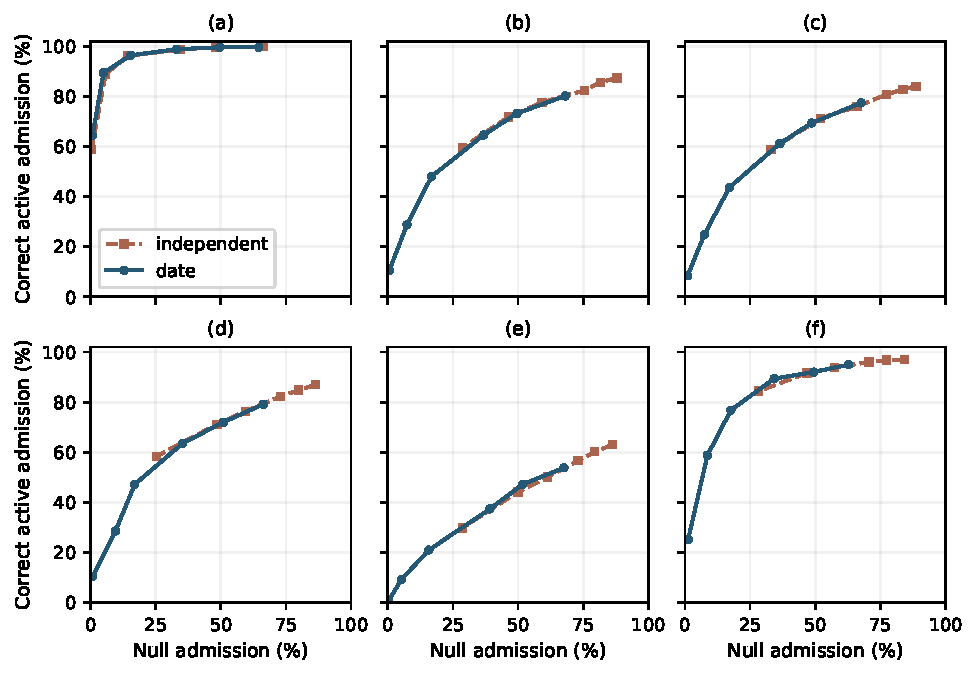
\includegraphics[width=0.98\linewidth]{figures/revised_gate_roc.pdf}
\caption{Revised gate trade-offs at EWMA span 60. Dashed lines with squares show
the independent-cell gate; solid lines with circles show the date-score gate.
Panels: (a) independent residuals, (b) correlated residuals, (c) duplicate
responses, (d) unequal histories, (e) heteroskedastic residuals and (f) changing
sign. Each panel uses 500 paired replications and thresholds 0.5, 0.75, 1, 1.5,
2 and 3. Smaller null admission
can trade off against active recovery; neither axis alone establishes superiority}
\label{fig:revised-gate}
\end{figure}


At approximately matched null-admission levels, recovery is similar for the
two screens in most cases. The evidence supports a correction for dependence
and duplicated responses, not a general improvement in the full estimator.
Threshold calibration in this experiment uses simulated null truth and is not
a practical error-control procedure for real data. The finite-span and changing-sign
cases are outside the asymptotic proposition.

Deterministic checks accompany the gate validation: repeating all members of a
fixed cluster equally leaves the score unchanged; observation masks and original-grid recency weights
are preserved. The complete-estimator comparison in
Section~\ref{sec:fitted-benchmark} uses equal weights and
independent dates, with its preprocessing repeated within each training fold.


\FloatBarrier

\section{Optional target and adaptive-weight specification}\label{app:adaptive}
When adaptive reweighting is off, $W_{kj}=A_k=A_{gj}=1$. When it is on,
the marginal magnitude weights are
%
\begin{equation} \label{eq:adapt-cell}
	W_{kj} \;=\; \frac{1}
	{\max\bigl(|\hat{\beta}_{j, \mathcal{C}(k)}|,\, \varepsilon\bigr)^{\gamma}},
\end{equation}
%
with exponent $\gamma>0$ and fixed stabilizer $\varepsilon>0$. A zero-pinned
cell is assigned placeholder weight one, which changes only a constant in the
objective. Let $\mathcal J_k$ contain the predictors of row $k$ that are not
pinned, and $\mathcal I_{gj}$ the members of block $(g,j)$ that are not pinned.
The implemented group weights are
\begin{equation}\label{eq:adapt-group}
	A_k=\left(\frac{\sum_{j\in\mathcal J_k}W_{kj}^2}
	{|\mathcal J_k|}\right)^{1/2},\qquad
	A_{gj}=\left(\frac{\sum_{k\in\mathcal I_{gj}}W_{kj}^2}
	{|\mathcal I_{gj}|}\right)^{1/2},
\end{equation}
with value one for an empty set. Thus adaptive group weighting can remain active
at $\alpha=0$; $\alpha=1$ removes the group term.

This magnitude-based construction is motivated by adaptive penalties
\citep{Zou:2006,Wang+Leng:2008}, but does not inherit their support or oracle
results. Fixed $\varepsilon$ bounds the weights. Moreover, a pooled marginal
slope need not vanish on a zero partial coefficient, even with uncorrelated
predictors when other members of its cluster are active. We make no
support-recovery or oracle-distribution claim for these fitted estimators.
The convex problem, numerical implementation and tuning protocol are described
in Section~\ref{app:computation}.


%% =====================================================================
\FloatBarrier


\section{Optional masked and weighted gate}\label{app:weighted-gate}

This appendix records optional software extensions of the gate. The complete
fitted estimator evaluated in the main text uses complete, equally weighted
observations; no missing-data fitting objective is proposed here. A validity
indicator $v_{tkj}$ is one only when response $k$ and predictor $j$ are both
observed. Missing pre-inception returns must not be passed as observed zeros.
For weights $w_t$, define
\begin{equation}
D_j=\sum_{t,k\in\mathcal C}w_tv_{tkj}x_{tj}^{2},\qquad
\widehat b_j=D_j^{-1}\sum_{t,k\in\mathcal C}w_tv_{tkj}x_{tj}y_{tk}.
\end{equation}
Equal weights remain the default of the optional \texttt{ewma\_span=None}
analytics. A finite span $s\geq1$ uses $w_t=(1-2/(s+1))^{T-t}$ on the original
row grid before masking. Gaps do not compress time. Inputs retain their caller's
centering convention; the sign routine introduces no extra intercept.

For overlapping response histories, use the date score
\begin{equation}
u_{tj}=w_tx_{tj}\sum_{k\in\mathcal C}v_{tkj}(y_{tk}-\widehat b_jx_{tj}),\qquad
\widehat V_j=\frac{n_{\mathrm{eff},j}}{n_{\mathrm{eff},j}-1}
\frac{\sum_tu_{tj}^{2}}{D_j^{2}}.\label{eq:weighted-date-score}
\end{equation}
Here $n_{\mathrm{eff},j}=(\sum_tw_ta_{tj})^2/\sum_tw_t^2a_{tj}$, where
$a_{tj}$ marks a date with the predictor and at least one response observed.
This effective count is over dates, not response cells. A zero $D_j$ supplies no
slope evidence and is excluded. For $D_j>0$, the score-sandwich
construction retains contemporaneous residual covariance \citep{CameronMiller2015};
using the effective-date multiplier is our finite-sample screening convention.
We apply Equation~\eqref{eq:gate} with $t_j=\widehat b_j/\sqrt{\widehat V_j}$.
Fewer than two effective dates cannot pass a positive gate. This statistic is
not asserted to have an exact Student distribution or multiplicity-adjusted
error control. Independent dates are assumed; serial dependence would require
an additional HAC or block treatment.

For a fixed cluster with masks and weights retained, repeating every member
$c$ times multiplies $D_j$ and $u_{tj}$ by $c$, so it
leaves both the slope and Equation~\eqref{eq:weighted-date-score} unchanged. In contrast,
the archived independent-cell standard error treats copies as added information.
Duplicating only one member of a heterogeneous cluster may change its weighting
and hence the pooled estimand; no invariance is claimed in that case or for
rerunning the clustering algorithm after duplication.

The design effect $1+(m-1)\rho_e$ and effective member count
$m/[1+(m-1)\rho_e]$ describe the balanced equal-variance special case derived
in Section~\ref{sec:theory}, with $\rho_e$ a marginal-regression residual
correlation. Unequal histories and recency weights require the masked scores
rather than a return-correlation adjustment. Missingness can also change the
population being averaged; the score formula does not correct informative
missingness. The consistency argument in Section~\ref{sec:theory} concerns
complete observations and equal weights.
They are not an extension to fixed-span EWMA: its effective temporal sample size
stays bounded as more history is stored. Marginal-versus-conditional sign
disagreement also remains possible after the variance repair.

These formulas describe screening only. Native-frequency routing, prior-target
sign overrides and missing-data fitting require additional definitions and
validation; they are outside the estimator studied here. The formulas also do
not include additional influence terms from estimating column scales, and no
calibrated variance assertion is made for that normalization.

\FloatBarrier

\section{The closed-form SSR identity} \label{app:ssr}
\subsection{Pooled-slope identity}\label{app:slope-identity}

We derive the sign of each coefficient from a univariate slope, pooled across the
responses that share a cluster. For predictor $j$, the pooled no-intercept slope
across all $N$ responses solves the first-order condition
$\bm{x}_j^\top \sum_{k=1}^{N} (\bm{y}_k - \hat{\beta}_j \bm{x}_j) = 0$, which gives
%
\begin{equation} \label{eq:slope-pooled}
	\hat{\beta}_j \;=\; \frac{\bm{x}_j^\top \bm{y}_{\mathrm{sum}}}
	{N\, \bm{x}_j^\top \bm{x}_j},
	\qquad
	\bm{y}_{\mathrm{sum}} \;\equiv\; \sum_{k=1}^{N} \bm{y}_k \;\in\; \mathbb{R}^T.
\end{equation}
%
Equation~\eqref{eq:slope-pooled} generalizes the single-response univariate slope
of \citet{Chatterjee+Hastie+Tibshirani:2025} to many responses, with the response
sum $\bm{y}_{\mathrm{sum}}$ in place of a single response. When the responses are
grouped into clusters, we compute the slope against the cluster-sum response and
broadcast it to every cluster member.
%
The cluster-specific expression is Equation~\eqref{eq:slope-cluster} in the main article.
%
Equation~\eqref{eq:slope-cluster} restricts Equation~\eqref{eq:slope-pooled} to
the cluster index set, and recovers it when $\mathcal{C} = \{1, \ldots, N\}$. The
cluster-pooled slope is the OLS slope of the cluster-mean response
$\bar{\bm{y}}_{\mathcal{C}} = |\mathcal{C}|^{-1} \bm{y}_{\mathcal{C}, \mathrm{sum}}$
on $\bm{x}_j$.

Broadcasting a pooled slope gives every member the same permitted direction.
This construction does not establish that their true partial coefficients have
that direction. Positive response correlation alone is insufficient, and a
cluster may contain both active and inactive responses for the same predictor.


\subsection{Residual identity}


This appendix derives the residual sum-of-squares identity of
Equation~\eqref{eq:ssr} and gives the full $t$~statistic.

\paragraph{Derivation.}
For predictor $j$, the pooled no-intercept slope $\hat{\beta}_j$ of
Equation~\eqref{eq:slope-pooled} satisfies the first-order condition
$\bm{x}_j^\top \bm{y}_{\mathrm{sum}} = N\, \hat{\beta}_j\, (\bm{x}_j^\top \bm{x}_j)$.
The pooled residual sum of squares aggregates the squared residuals of the $N$
per-response fits at the common slope $\hat{\beta}_j$,
%
\begin{align}
	\mathrm{SSR}_j
	&= \sum_{k=1}^{N} \bigl\| \bm{y}_k - \hat{\beta}_j\, \bm{x}_j \bigr\|_2^2
	= \sum_{k=1}^{N} \Bigl( \|\bm{y}_k\|_2^2
	- 2\, \hat{\beta}_j\, \bm{x}_j^\top \bm{y}_k
	+ \hat{\beta}_j^{\,2}\, \bm{x}_j^\top \bm{x}_j \Bigr) \notag \\
	&= \|\bm{Y}\|_F^2
	- 2\, \hat{\beta}_j\, \bm{x}_j^\top \bm{y}_{\mathrm{sum}}
	+ N\, \hat{\beta}_j^{\,2}\, \bm{x}_j^\top \bm{x}_j , \label{eq:ssr-expand}
\end{align}
%
using $\sum_k \|\bm{y}_k\|_2^2 = \|\bm{Y}\|_F^2$ and
$\sum_k \bm{x}_j^\top \bm{y}_k = \bm{x}_j^\top \bm{y}_{\mathrm{sum}}$.
Substituting the first-order condition
$\bm{x}_j^\top \bm{y}_{\mathrm{sum}} = N\, \hat{\beta}_j (\bm{x}_j^\top \bm{x}_j)$
into the middle term gives the closed-form identity
\begin{equation}\label{eq:ssr}
\mathrm{SSR}_j = \|\bm{Y}\|_F^2 - N\,\hat\beta_j^{\,2}
(\bm{x}_j^\top\bm{x}_j).
\end{equation}
This is an algebraic identity; it does not justify a variance formula under
dependence or heterogeneous effects.
The right-hand side requires only $\|\bm{Y}\|_F^2$ (computed once), the
per-predictor inner product $\bm{x}_j^\top \bm{x}_j$, and the slope, so the full
$(N, M)$ statistic is one matrix product rather than a loop that forms the
$T \times N$ residual matrix for each predictor.

\paragraph{Archived independent-cell statistic.}
The archived experiments use the following residual scale and screening
statistic:
%
\begin{equation} \label{eq:tstat}
	\hat{\sigma}_j^{\,2} = \frac{\mathrm{SSR}_j}{N\, T - N},
	\qquad
	\widehat{\mathrm{SE}}\bigl(\hat{\beta}_j\bigr) =
	\sqrt{\frac{\hat{\sigma}_j^{\,2}}{N\, \bm{x}_j^\top \bm{x}_j}},
	\qquad
	t_j = \frac{\hat{\beta}_j}{\widehat{\mathrm{SE}}\bigl(\hat{\beta}_j\bigr)}.
\end{equation}
%
The cluster-pooled variant substitutes $|\mathcal C|$ for $N$ and restricts the
Frobenius norm to cluster columns. The denominator $NT-N$ is the historical
screening convention retained to identify those results; no exact Student
reference distribution is assigned to it. The SSR includes discrepancies
between each response and the common pooled slope, including between-response
slope heterogeneity. It does not estimate the cross-response covariance terms
in Equation~\eqref{eq:pooling-variance}. In particular, independent full-model
errors do not justify treating marginal residuals as independent cells.

The revised statistic uses Equation~\eqref{eq:date-score}, which squares the
sum of residual scores within a date. For a prespecified cluster, complete
observations, equal weights and fixed analysis scales, it is the
heteroskedasticity-robust slope variance for regression on the cluster-mean
response, with the stated finite-sample multiplier. With sample-estimated
column scales, the following proposition uses its positive score-scale limit
without identifying it as the full sampling variance of the normalized slope.
It is this statistic, rather than Equation~\eqref{eq:tstat}, that the
proposition covers.


\FloatBarrier

\section{Clustering conventions}\label{app:clustering-conventions}

The partition can be supplied externally or estimated from training responses.
The revised fitted-estimator experiments use $D_{kl}=\sqrt{2(1-C_{kl})}$ with
$\bm C=\operatorname{corr}(\bm Y)$, the Euclidean distance between centered
response vectors normalized to unit length, and Ward linkage on these
distances. This interpretation requires correlations computed from a common
observation grid. Arbitrary pairwise-missing correlations need not define a
Euclidean configuration, and a monotone transformation of the distances does
not in general preserve Ward's tree. The cut is a predeclared fraction of the
final Ward merge height, $0.5$ in the synthetic benchmark and $0.7$ in the
nested eQTL analysis. Under this rule a fraction of one produces a single
cluster, while small positive cuts need not produce all singletons when
distances are zero. A target number of clusters is an alternative cut rule and
is stated when used. The cut fraction is a user-selected hyperparameter, so
the partition depends on both data and tuning choices, and none of these
constructions guarantees agreement of partial coefficient signs within a
discovered cluster.

The companion software manuscript and the synthetic teaching examples of
Section~\ref{app:variance-sensitivity} use the package's own convention, Ward
linkage applied to $1-C_{kl}$ with a distance cut at a fraction of the largest
pairwise distance. That transform is a squared-distance heuristic rather than
a Ward sum of squared deviations, and its partitions are not interchangeable
with those of the revised protocol. The record of the historical experiments
and of the superseded eQTL analysis is kept with the replication materials in
Online Resource~2.

\bibliographystyle{sn-basic}
\bibliography{refs}
\end{document}
